\section{Physical Simulation Studies}
%% TODO - channel level heatmap for neutrino event

We now discuss the methodologies of the physical simulations used as input to the digital tile simulation described in the previous section.

\subsection{Simulated Detector Properties}


%%
\subsection{Radiogenic Backgrounds as a Calibration Source}

\begin{figure}[]
\centering
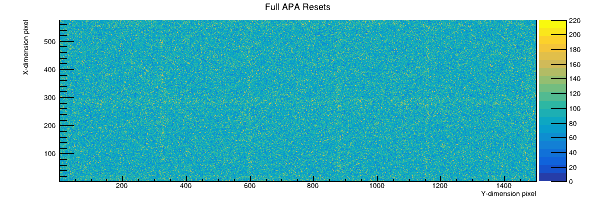
\includegraphics[width=\textwidth]{images/fullApaResets.png}
\caption{Full 1000 second of radiogenic background source simulation input into all pixels within the APA.}
\end{figure}~\label{fig:background_simulation}

\begin{figure}[]
\centering
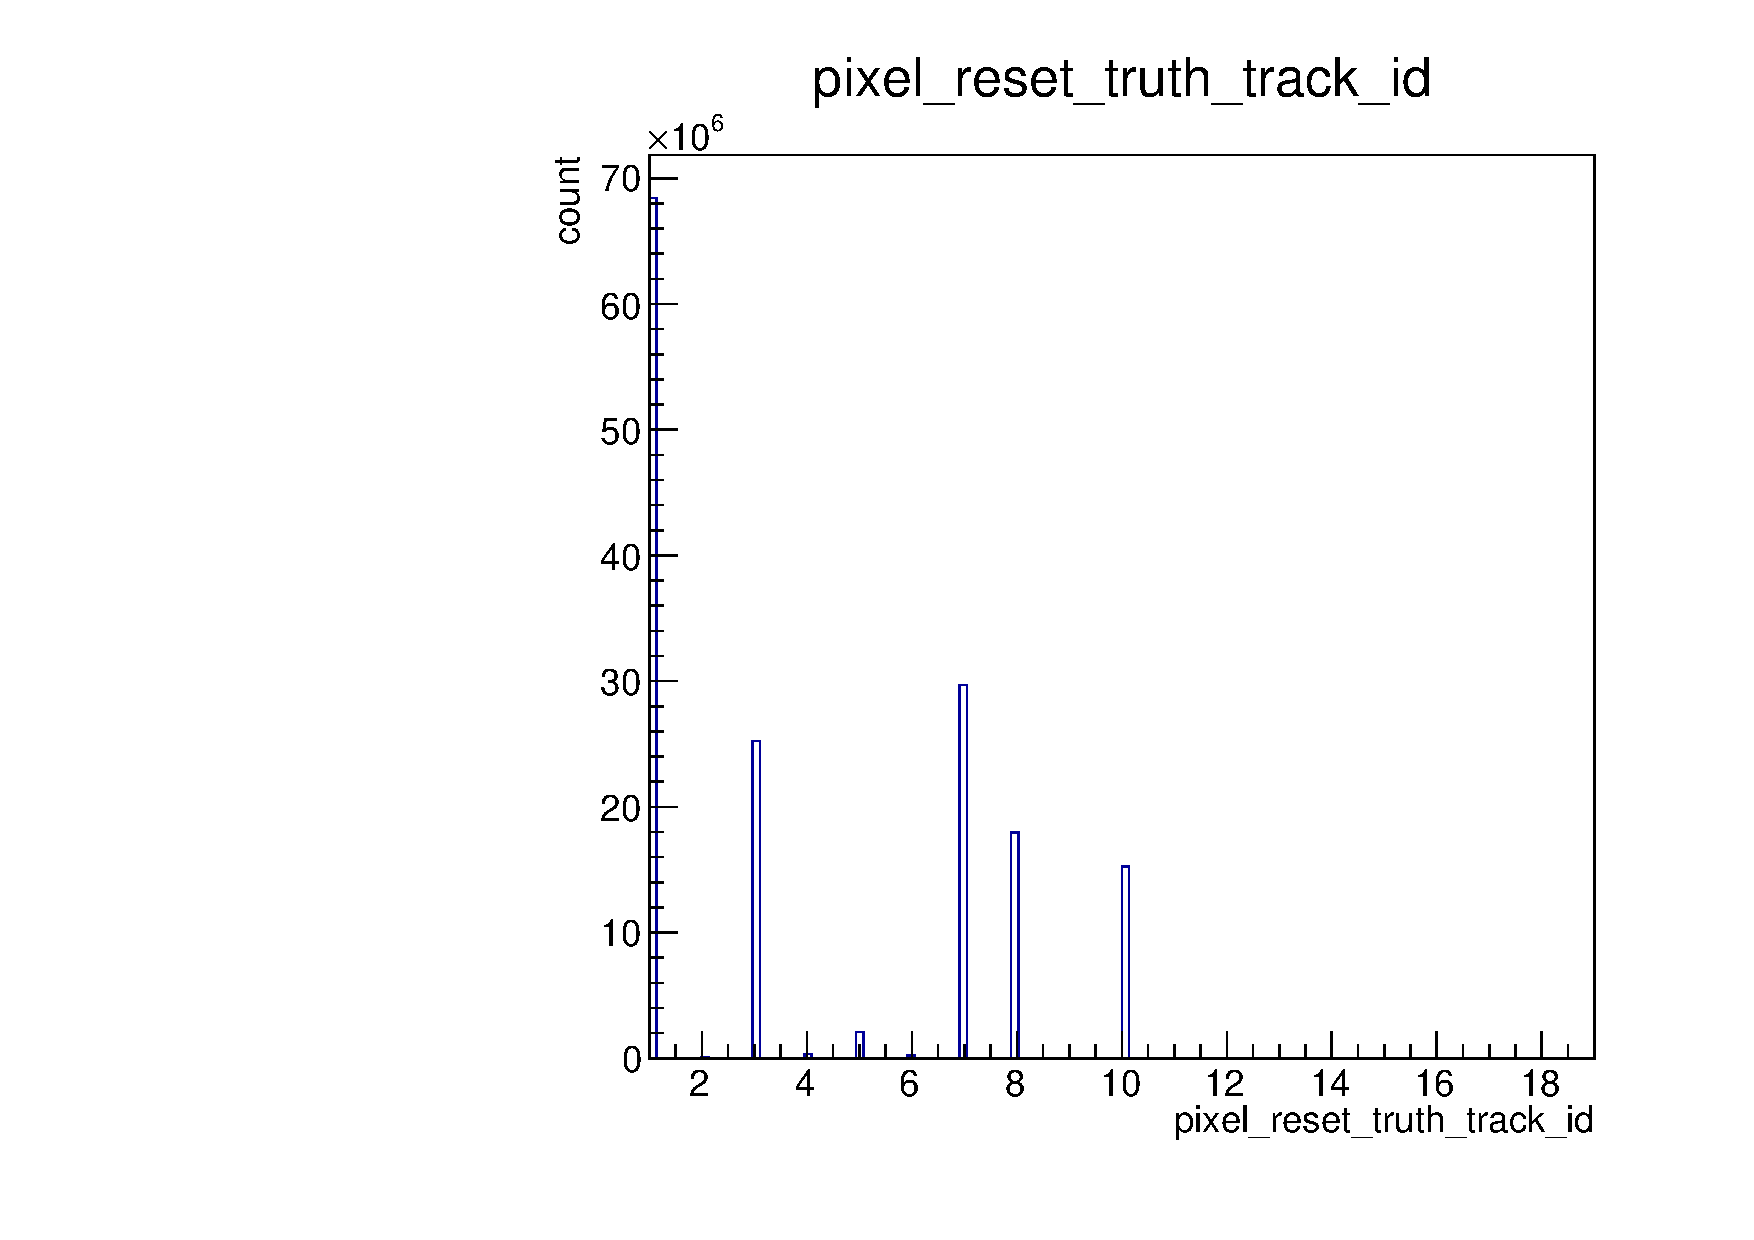
\includegraphics[width=\textwidth]{images/pixel_reset_truth_track_id.pdf}
\caption{}
\end{figure}~\label{fig:pixel_track_id}

\begin{figure}[]
\centering
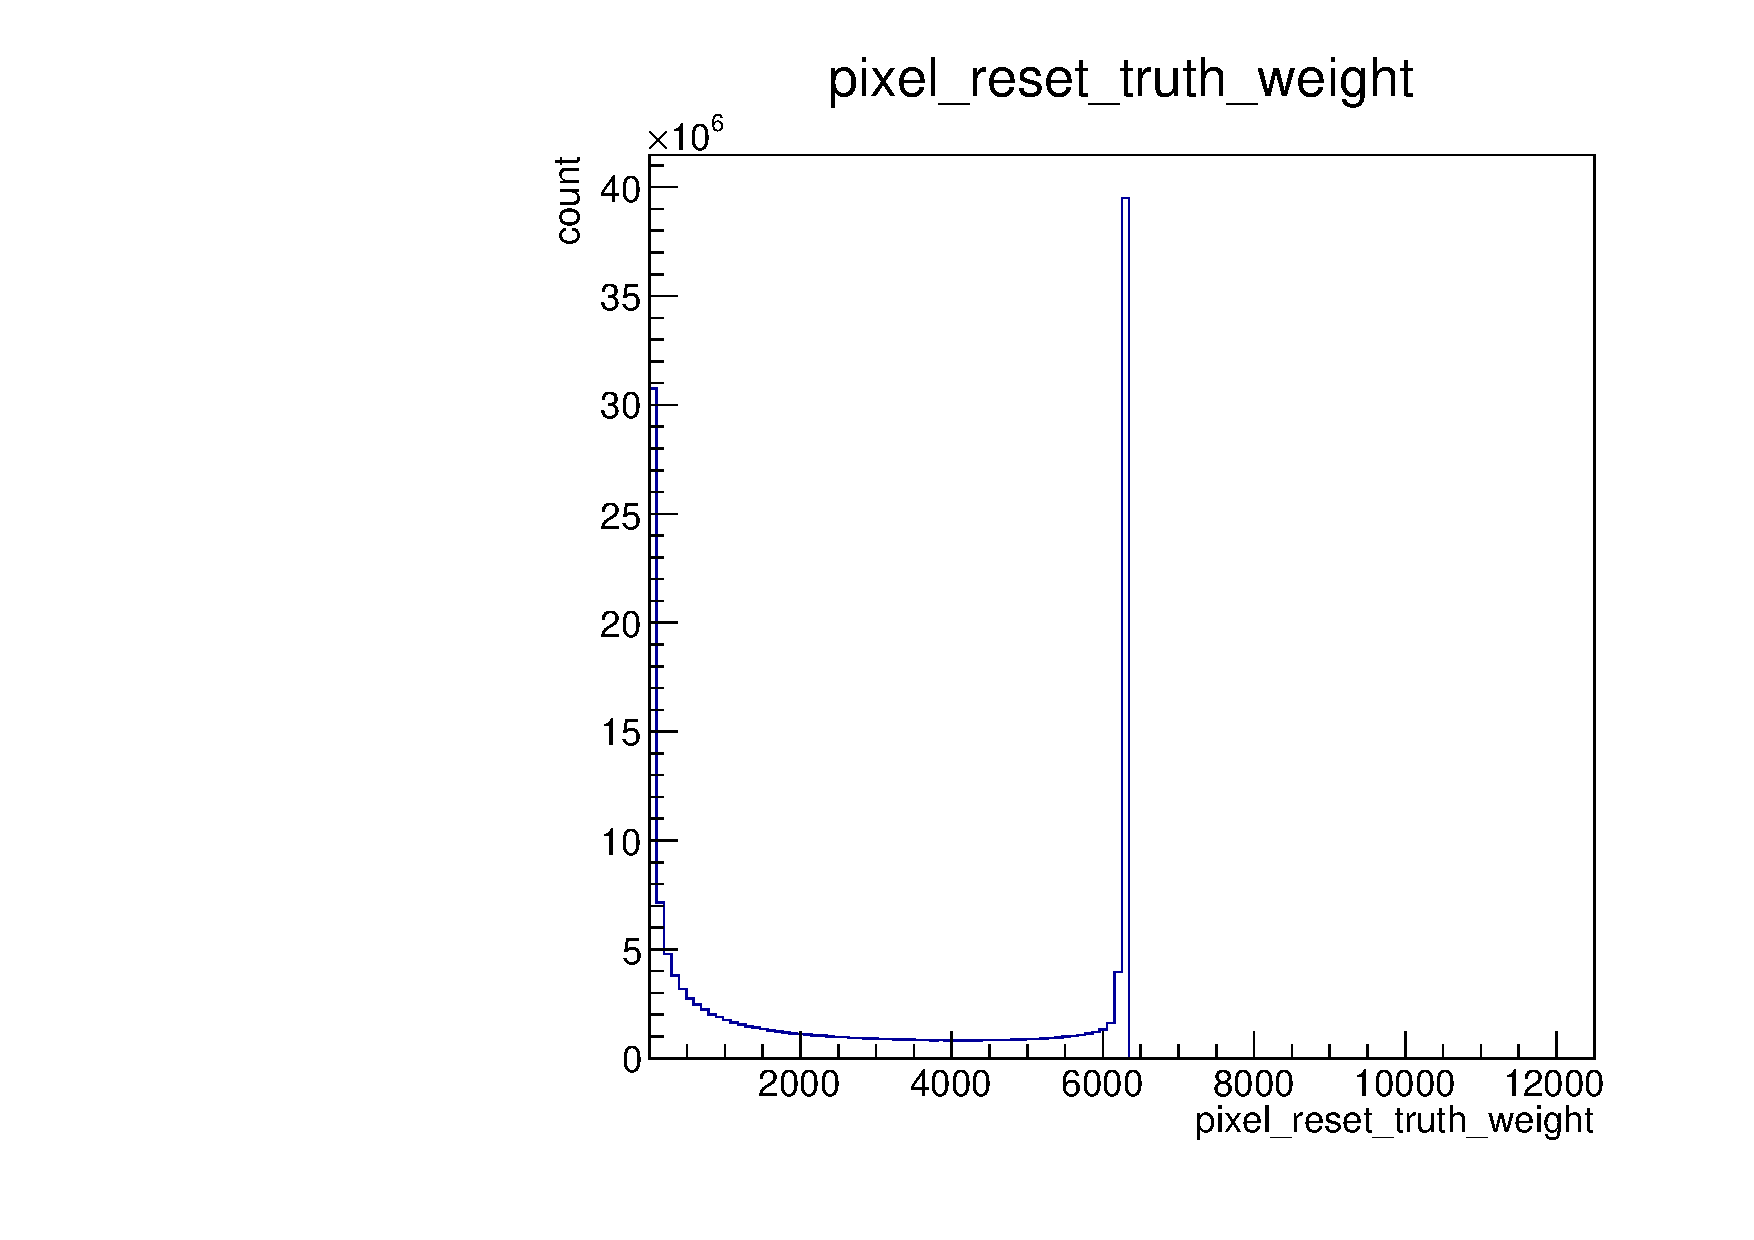
\includegraphics[width=\textwidth]{images/pixel_reset_truth_weight.pdf}
\caption{Truth weight of the individual resets for all combined resets in a 1000 s APA run.}
\end{figure}~\label{fig:pixel_truth_weight}


\begin{figure}[]
\centering
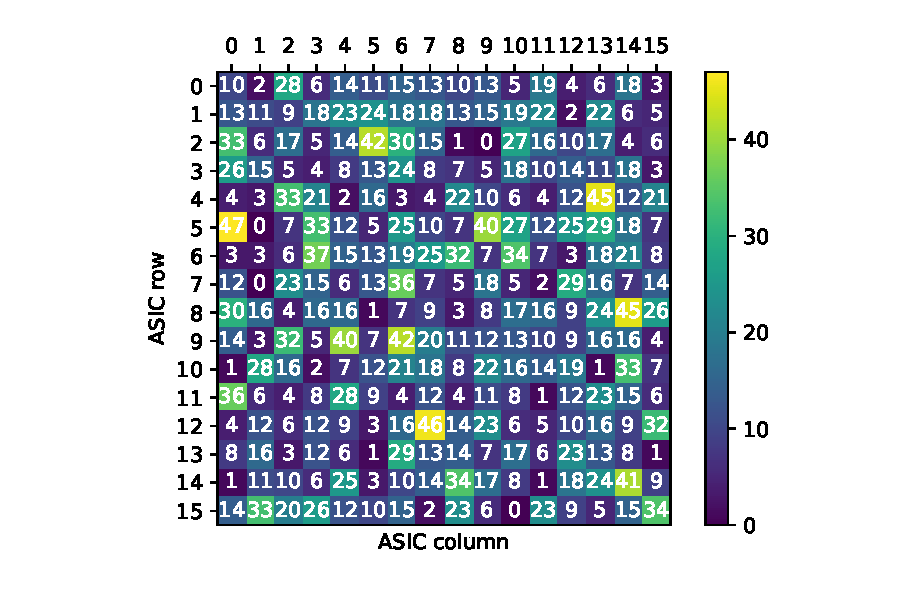
\includegraphics[width=\textwidth]{images/localHitsRadiogenic.pdf}
\caption{Baseline noise input for the digital simulation from all radiogenic sources and background leakage current.}
\end{figure}~\label{fig:reference_input_noise}

%% example local vs remote of snake
\begin{figure}
\centering
\begin{subfigure}{.5\textwidth}
  \centering
  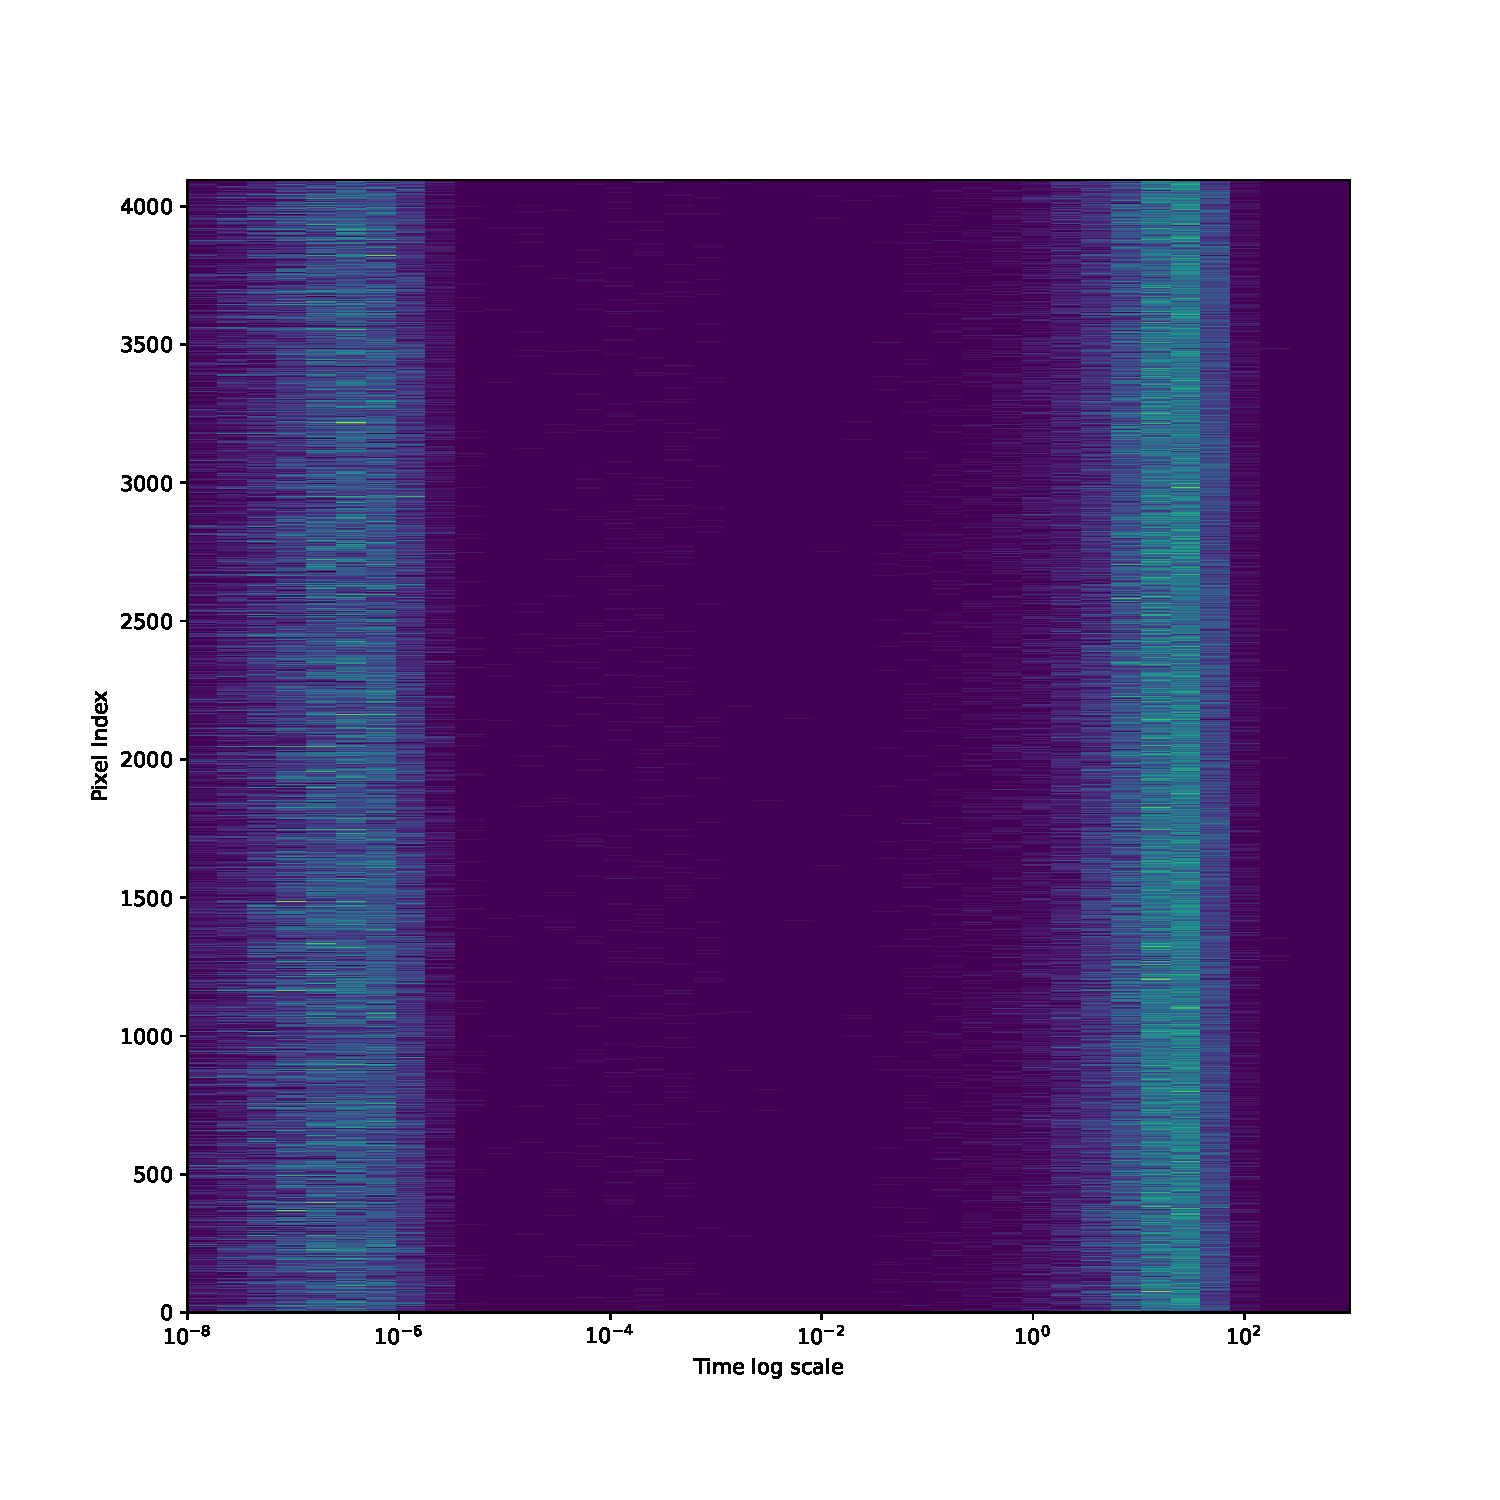
\includegraphics[width=\textwidth]{images/radiogenicRTDtimescale.pdf}
  \caption{4096 Pixel Resets in log scale of time.}
\end{subfigure}%
\begin{subfigure}{.5\textwidth}
  \centering
  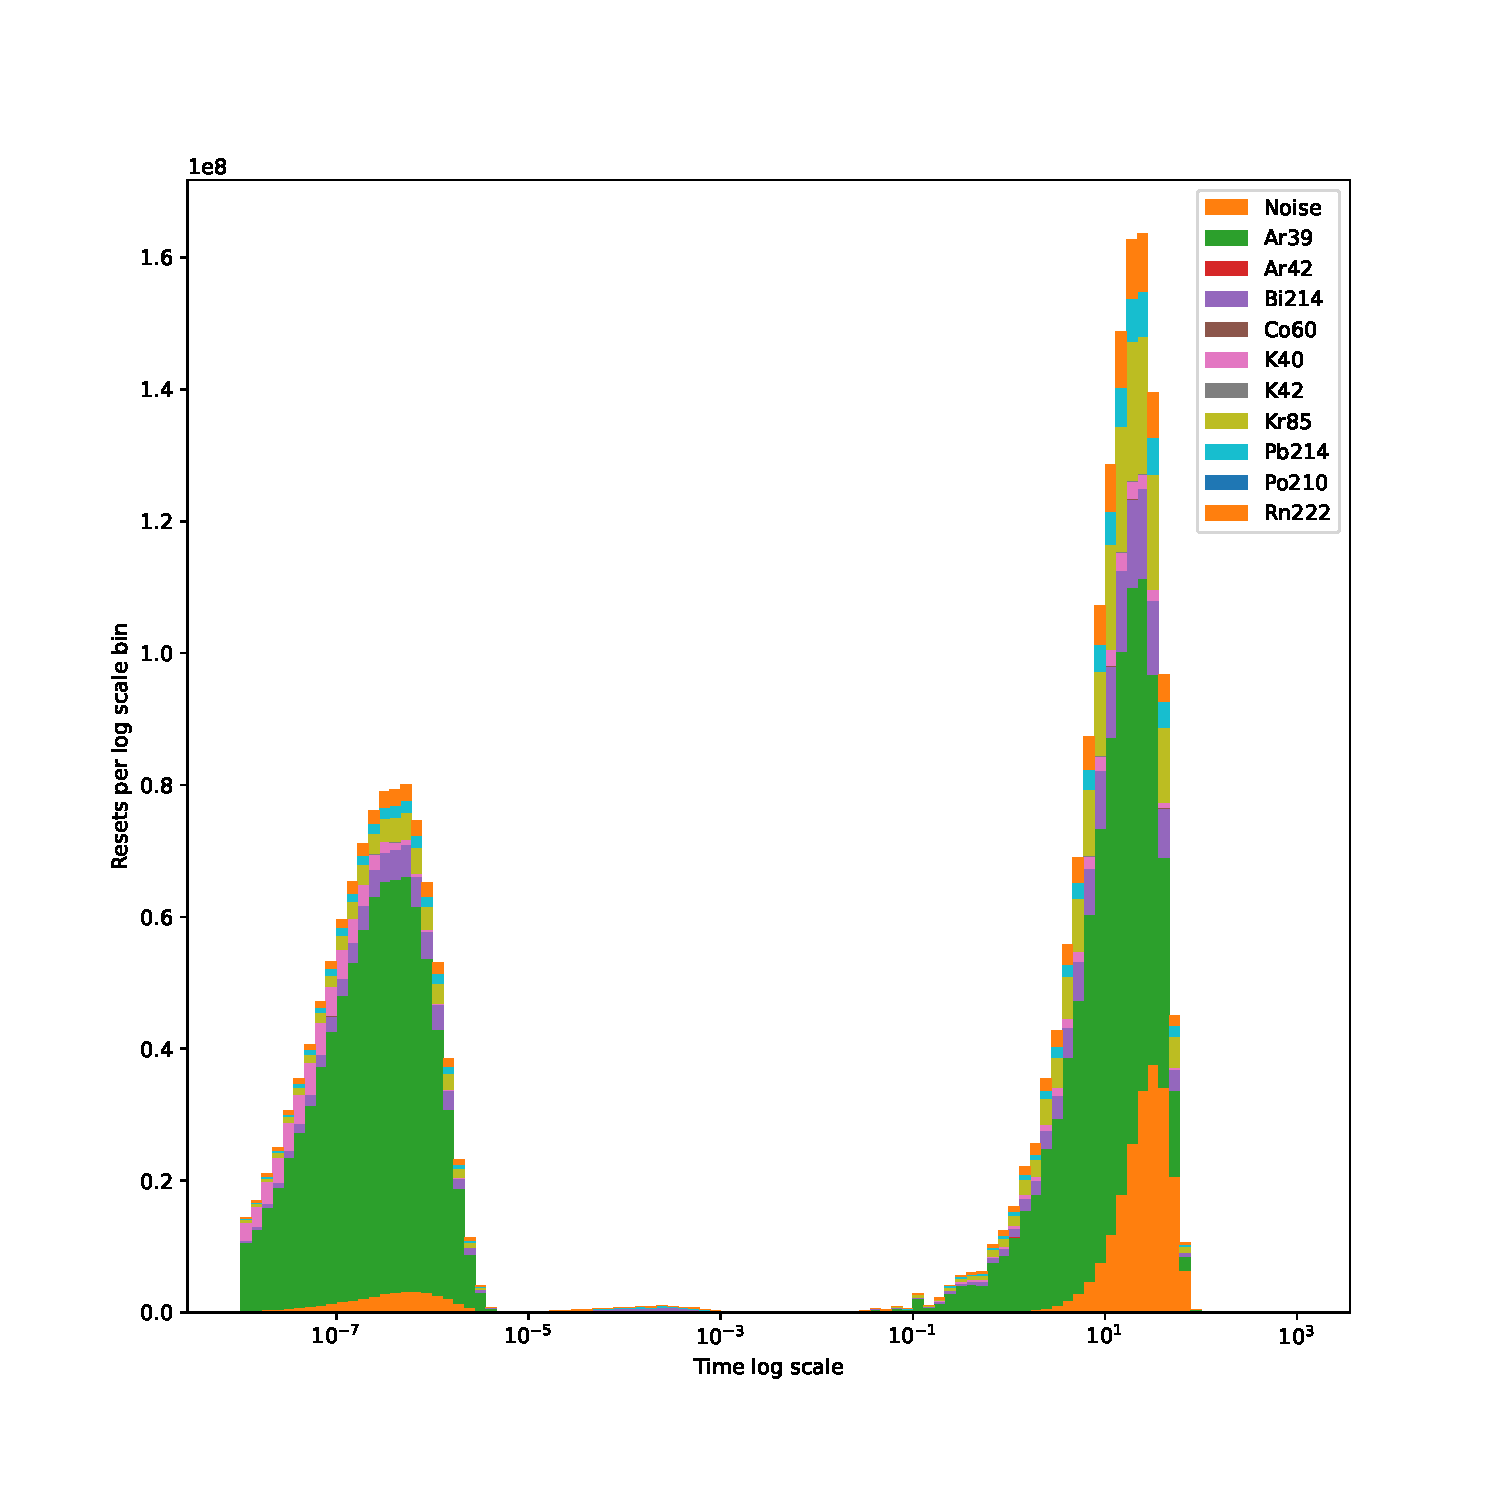
\includegraphics[width=\textwidth]{images/radiogenicRTDtimescale_stack_1d_noise.pdf}
  \caption{Flattend histogram against time}
\end{subfigure}
\caption{all 4096 pixels in a 16$\times$16 array for 1000 seconds of radiogenic data. 
There are two clusters of resets on two different time scales.}
~\label{fig:radiogenic_rtd_timescales}
\end{figure}

\begin{figure}
\centering
\begin{subfigure}{.5\textwidth}
  \centering
  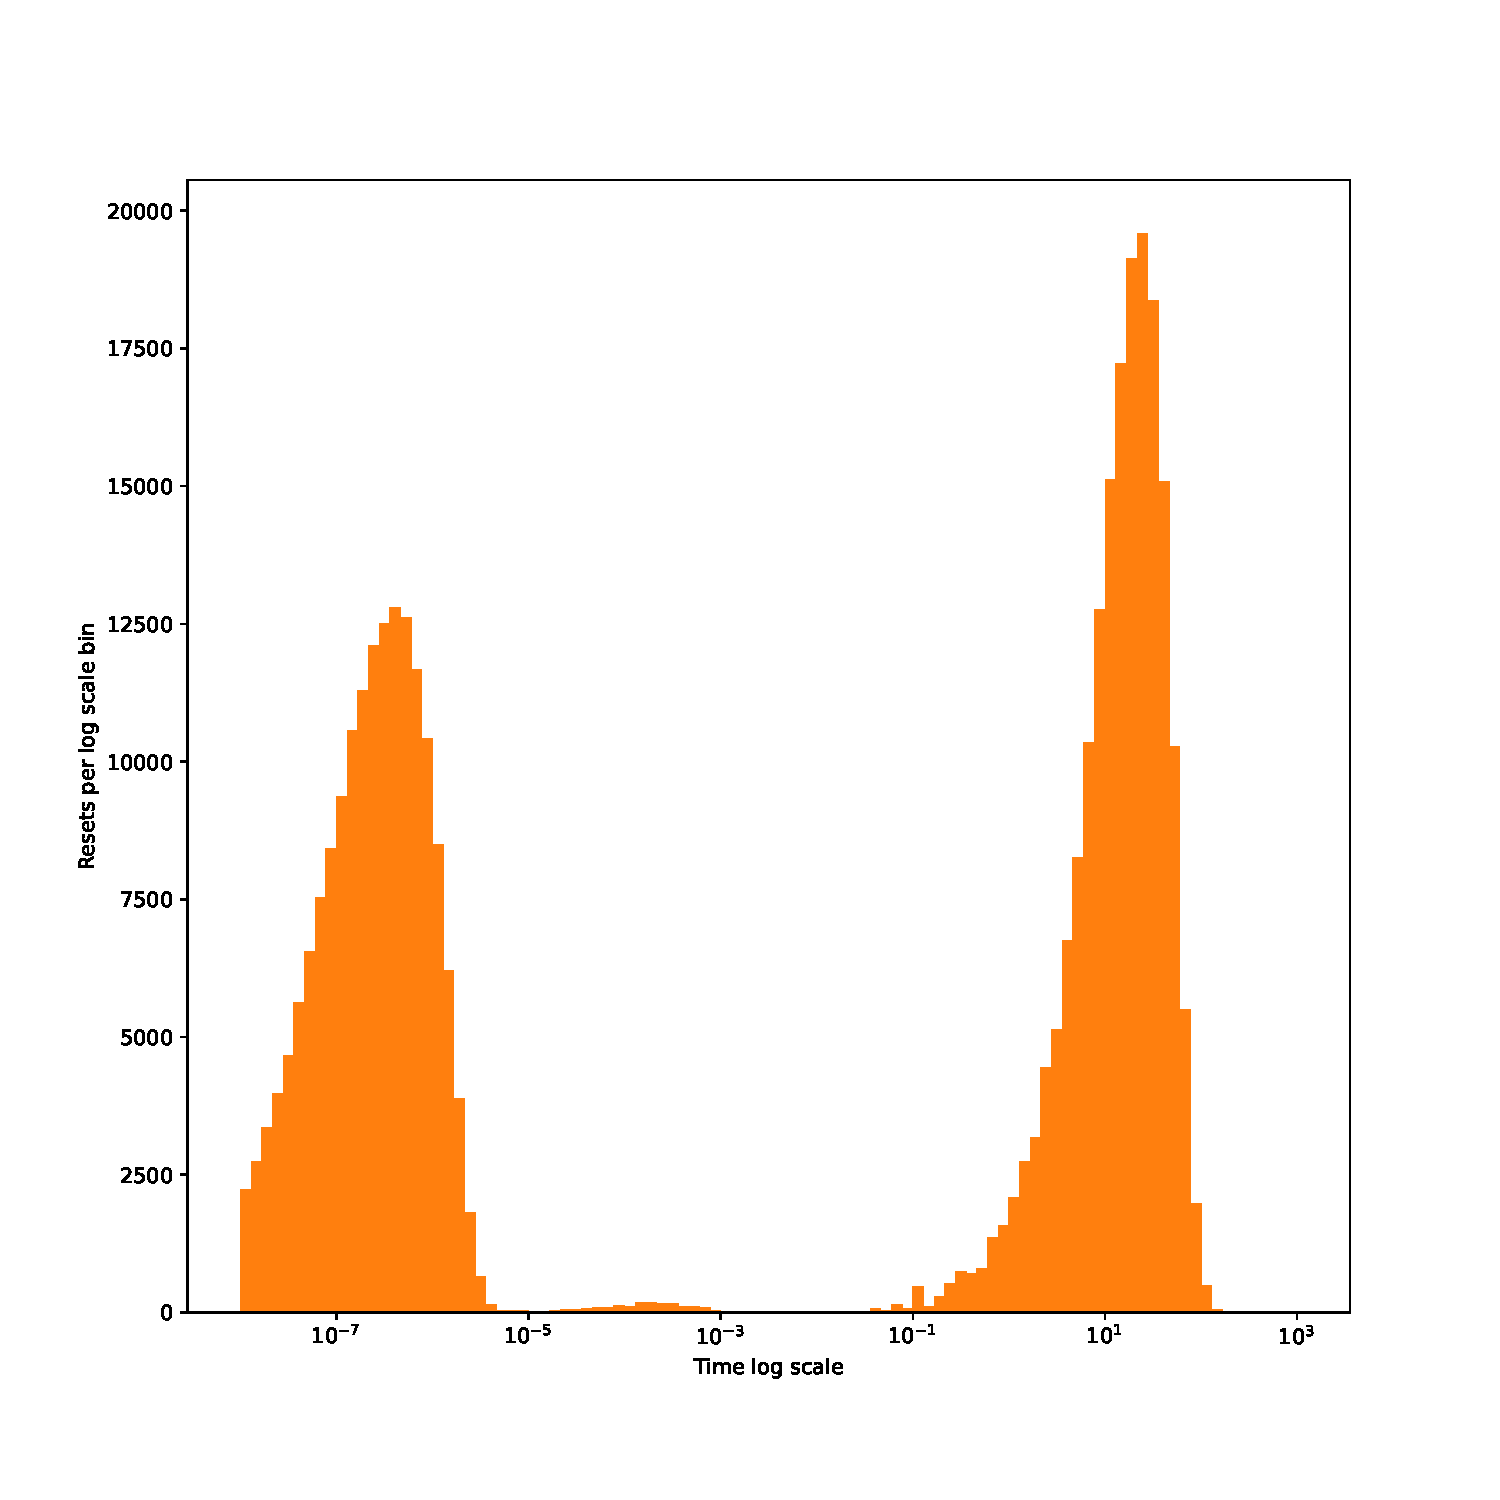
\includegraphics[width=\textwidth]{images/radiogenicRTDtimescale_1d.pdf}
  \caption{4096 Pixel Resets in log scale of time.}
\end{subfigure}%
\begin{subfigure}{.5\textwidth}
  \centering
  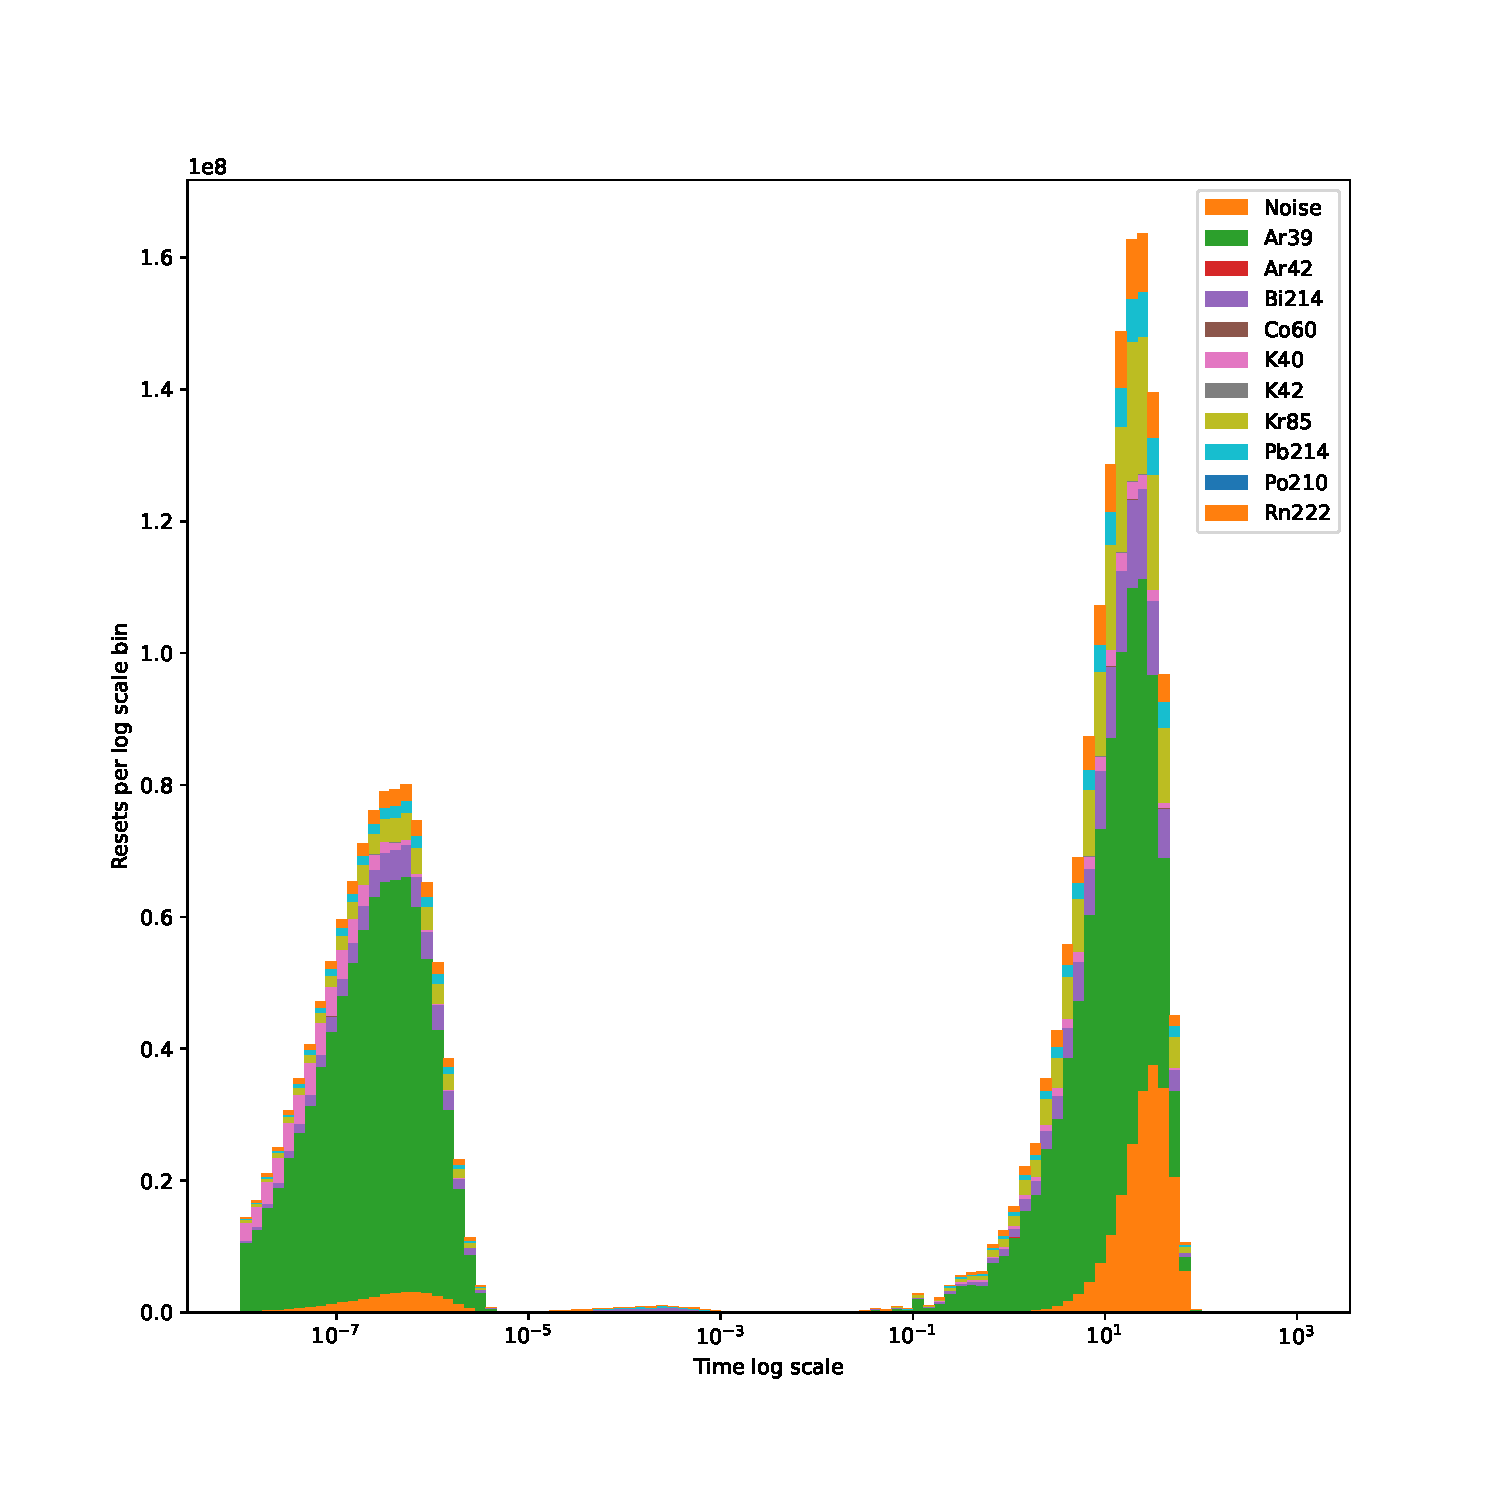
\includegraphics[width=\textwidth]{images/radiogenicRTDtimescale_stack_1d_noise.pdf}
  \caption{Flattend histogram against time}
\end{subfigure}
\caption{all 4096 pixels in a 16$\times$16 array for 1000 seconds of radiogenic data. 
There are two clusters of resets on two different time scales.}
~\label{fig:radiogenic_rtd_timescales_comparing_no_noise}
\end{figure}

sources of backgrounds are taken from~\citep{DUNE-FD_TDRv4:Abi_2020}
Radiological Backgrounds~\citep{ar39_backgrounds, phd_backgrounds}

%% list of sources here
We use the following list of radiogenic sources of 10 separate iterations of runs of 1000 seconds.

\begin{table}
\begin{center}
\begin{tabular}{|c c c c c c|}
 \hline
 Isotope & Rate [Bq/kg] & Region & Region Mass [kg] & Rate [Bq] & Number of Decays (per 10 s window) \\ [0.5ex]
 \hline\hline
  $^{210}$Po & 0.2 & PD [Bq/$m^2$] & 2.46856 & 0.493712 & 5 \\
  $^{60}$Co & 0.0455 & CPA & 90 & 4.095 & 41 \\
  $^{40}$K & 0.49 & APA & 258 & 1,264.2 & 12,642 \\
  $^{39}$Ar & 1.010 & bulk LAr & ~70,000 & 70,700 & 707,000 \\
  $^{42}$Ar & 0.000092 & bulk LAr & ~70,000 & 6.44 & 64 \\
  $^{42}$K  & 0.000092 & bulk LAr & ~70,000 & 6.44 & 64 \\
  $^{222}$Rn & 0.04 & bulk LAr & ~70,000 & 2800 & 28,000 \\
  $^{214}$Pb & 0.01 & bulk LAr & ~70,000 & 700 & 7,000 \\
  $^{214}$Bi & 0.01 & bulk LAr & ~70,000 & 700 & 7,000 \\
  $^{85}$Kr & 0.115 & bulk LAr & ~70,000 & 8050 & 80,500 \\
 \hline
\end{tabular}
\caption{The radiogenic background distribution is the same as that found in previous work~\citep{qpix:shion}.}
\end{center}
\end{table}
~\label{table:radiogenic_backgrounds}

%%

\subsection{Reset Distribution of Sources}

%% graphic for reset distribution from sources

%% graphic for energy deposited by source

%%%%%%%%%%%%%%%%%%%%%%%%%%%%%%%%%%%%%%%%%%%%%%%%%%%%%%%%%%%%%%%%%%%%%%%%%%%%%%%%
%%%%%%%%%%%%%%%%%%%%%%%%%%%%%%%   Part 2   %%%%%%%%%%%%%%%%%%%%%%%%%%%%%%%%%%%%%
%%%%%%%%%%%%%%%%%%%%%%%%%%%%%%%%%%%%%%%%%%%%%%%%%%%%%%%%%%%%%%%%%%%%%%%%%%%%%%%%
\section{Neutrino Beam High Energy Studies}~\label{sec:neutrino_studies}

Here we discuss the verification of the digital framework within the high energy regime.
For this we use as an input source neutrino events from the FNAL accelerate

\begin{figure}[]
\centering
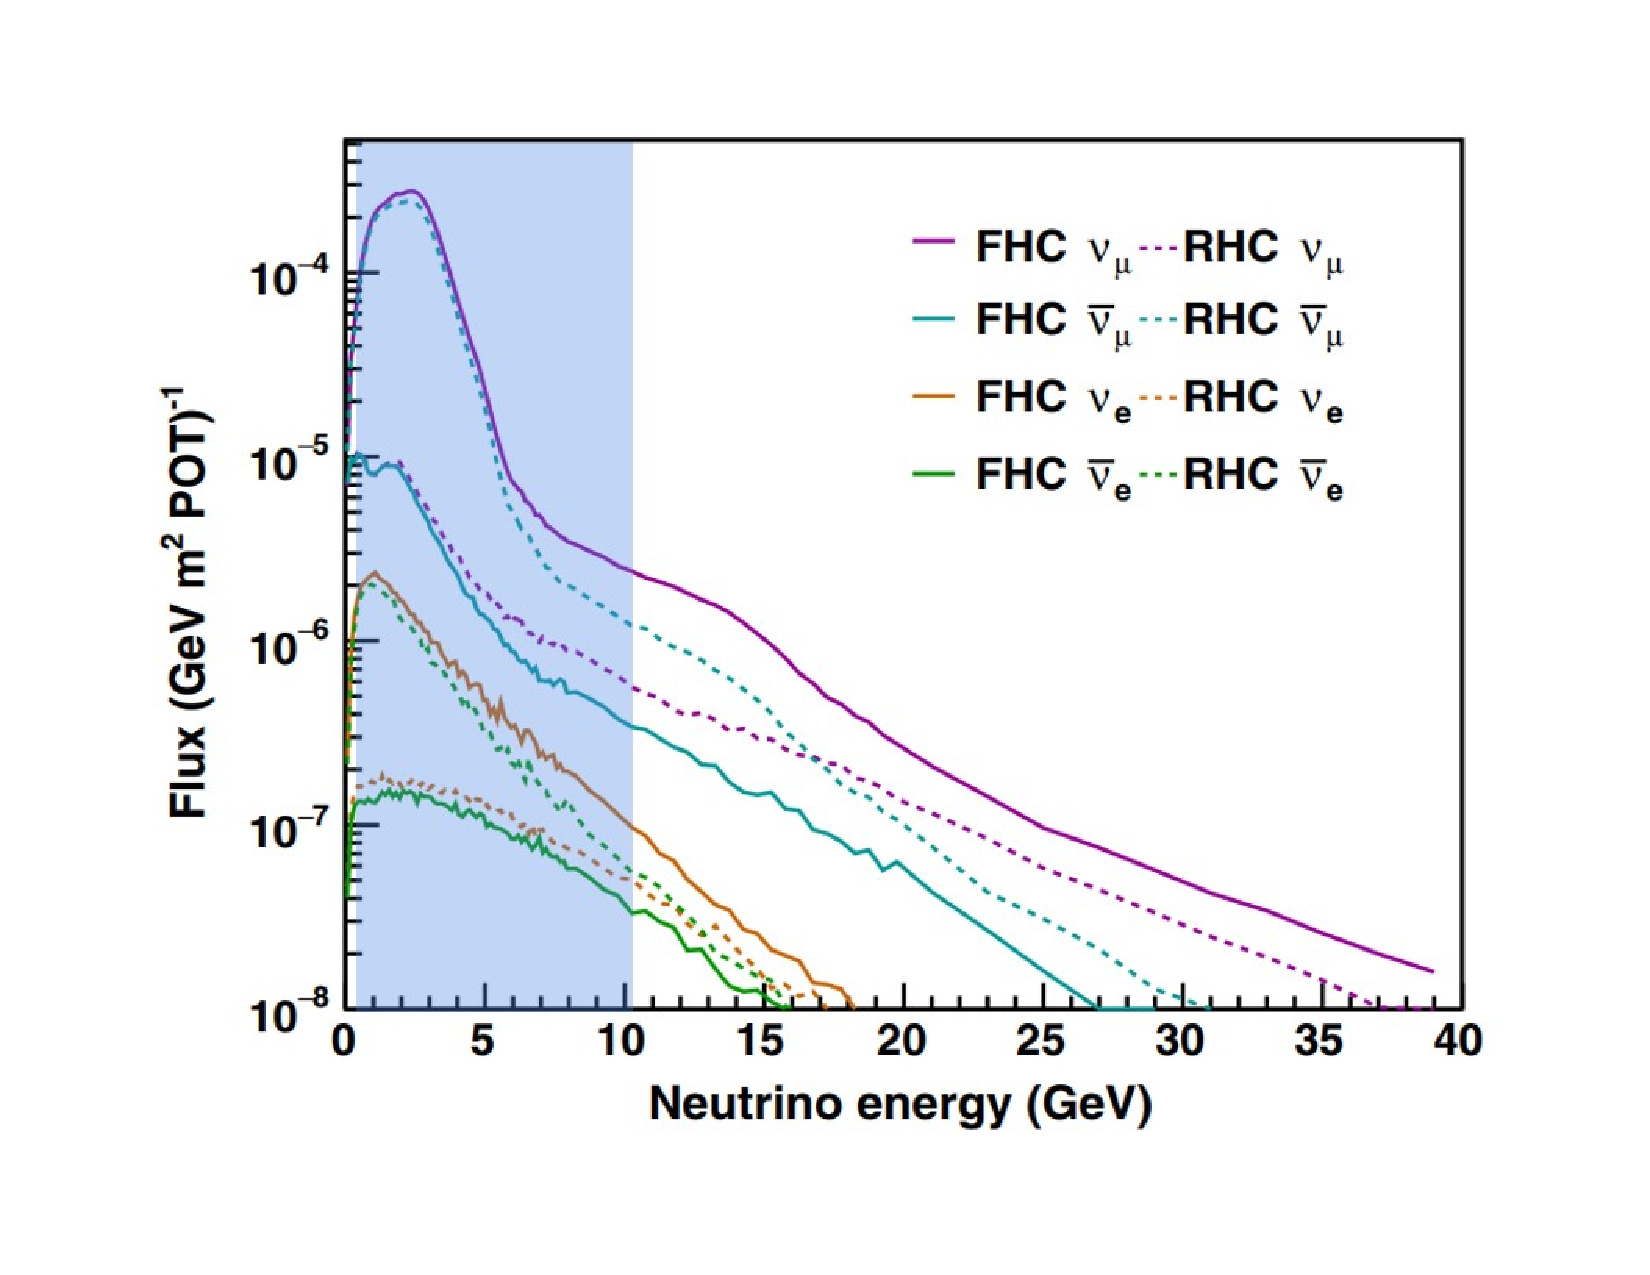
\includegraphics[width=\textwidth]{images/dune_flux_energy_range.pdf}
\caption{Flux spectrum of neutrinos from the neutrino beam used in this study. This figure is taken from~\cite{electron_flux_image_2020}.}
\end{figure}~\label{fig:neutrino_flux}

%% TODO - Citation of the beam here

%% DUNE-FD TDR specification citation here
The DUNE-FD Vol.2 TDR~\citep{DUNE_FD_TDRv2_2020} describes in detail the design requirements for a future single-phase module.


%% fig example neutrino event

%% fig example neutrino pixelated event

%%

\subsection{Neutrino Event Parameters}

The parameters used to vary the tiles for these neutrino input energies are shown on Table~\ref{table:tile_params}.


\begin{table}
\begin{center}
\begin{tabular}{|| p{30mm} | p{30mm} | p{90mm} ||}
 \hline
 Name & Values & Relation \\ [0.5ex]
 \hline\hline
  Neutrino Energy & 0.25~GeV to 10~GeV, in steps of 0.25GeV & neutrino energy determines output secondary energy, which causes more resents and directly affects buffer depths. \\
 \hline
  Neutrino Type & $\nu_{e}$, $\bar{\nu_{e}}$, $\nu_{\mu}$, $\bar{\nu_{\mu}}$ & Oscillation measurements require a measurement of electron flavor neutrino appearance, and muon disappearance.\\
 \hline
  Horn Current & Forward and Reverse & Beam horn current selection affects which neutrino is present. \\
 \hline
  Z-position & 10\unit{cm}, 80\unit{cm}, 180\unit{cm}, 280\unit{cm}, 350\unit{cm}  & Interaction z-position above the anode plane. \\
 \hline
  Momentum Angle & 0\unit{\degree}, $\pm$2\unit{\degree}, $\pm$90\unit{\degree} & Different momentum angles are different Z-positions give larger track lengths within the active volume. \\
 \hline
\end{tabular}
\caption{The different neutrino simulation parameters which are passed into Geant4 based simulation.
  The original interaction products are created using GENIE~\citep{Andreopoulos:2009rq}.
  The output products from this generator are then configured using the different parameters described above.
}
\end{center}
\end{table}
~\label{table:neutrino_params}

\subsection{Neutrino Event Results}

% lego plot of all of the events

% image example th2i of a single event in the full APA


% image example of a full waveform
 
%% example integral of ASIC buffer depths with constant theta
\begin{figure}
\centering
\begin{subfigure}{.5\textwidth}
  \centering
  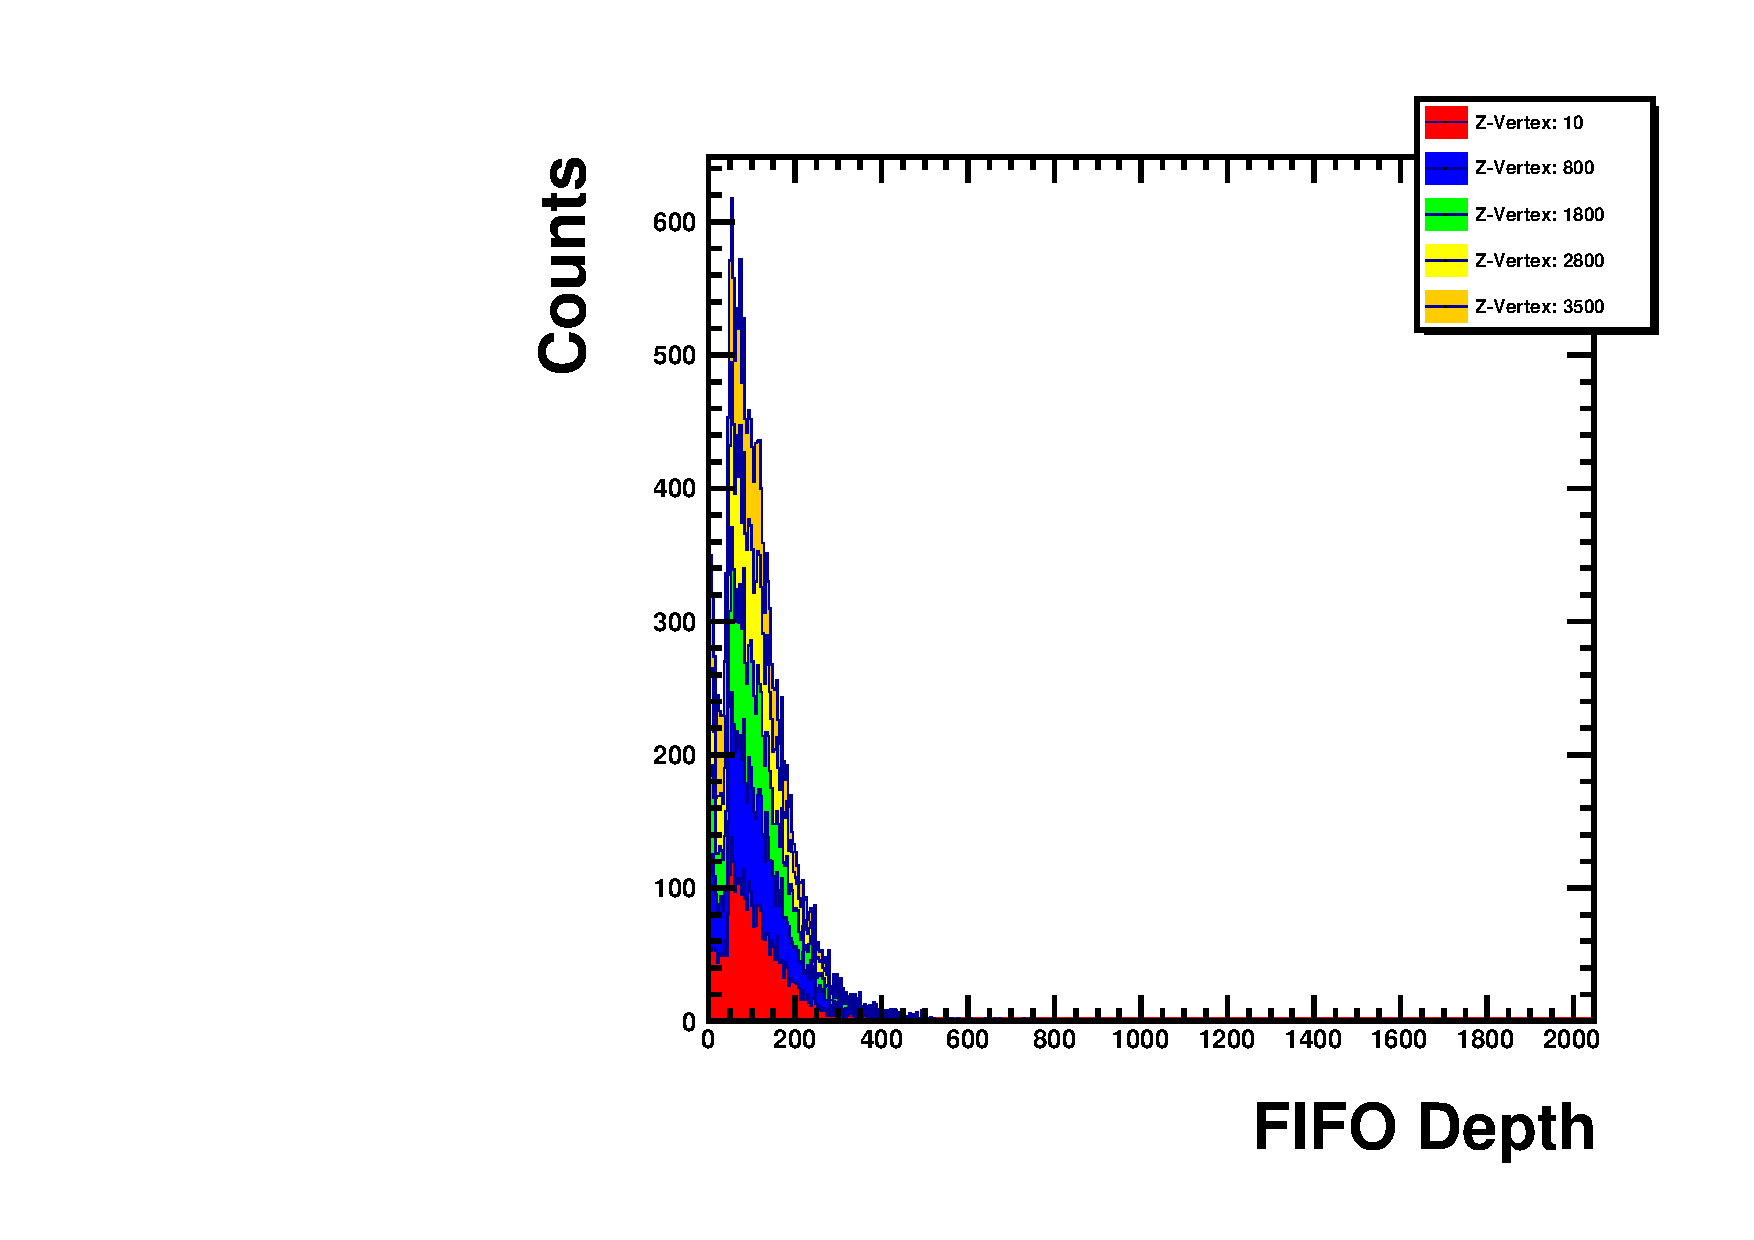
\includegraphics[width=\textwidth]{images/Const_Theta0_ASIC_stack_integral_pdg12_fhc.pdf}
  \caption{Stack of ASIC local FIFO depths}
\end{subfigure}%
\begin{subfigure}{.5\textwidth}
  \centering
  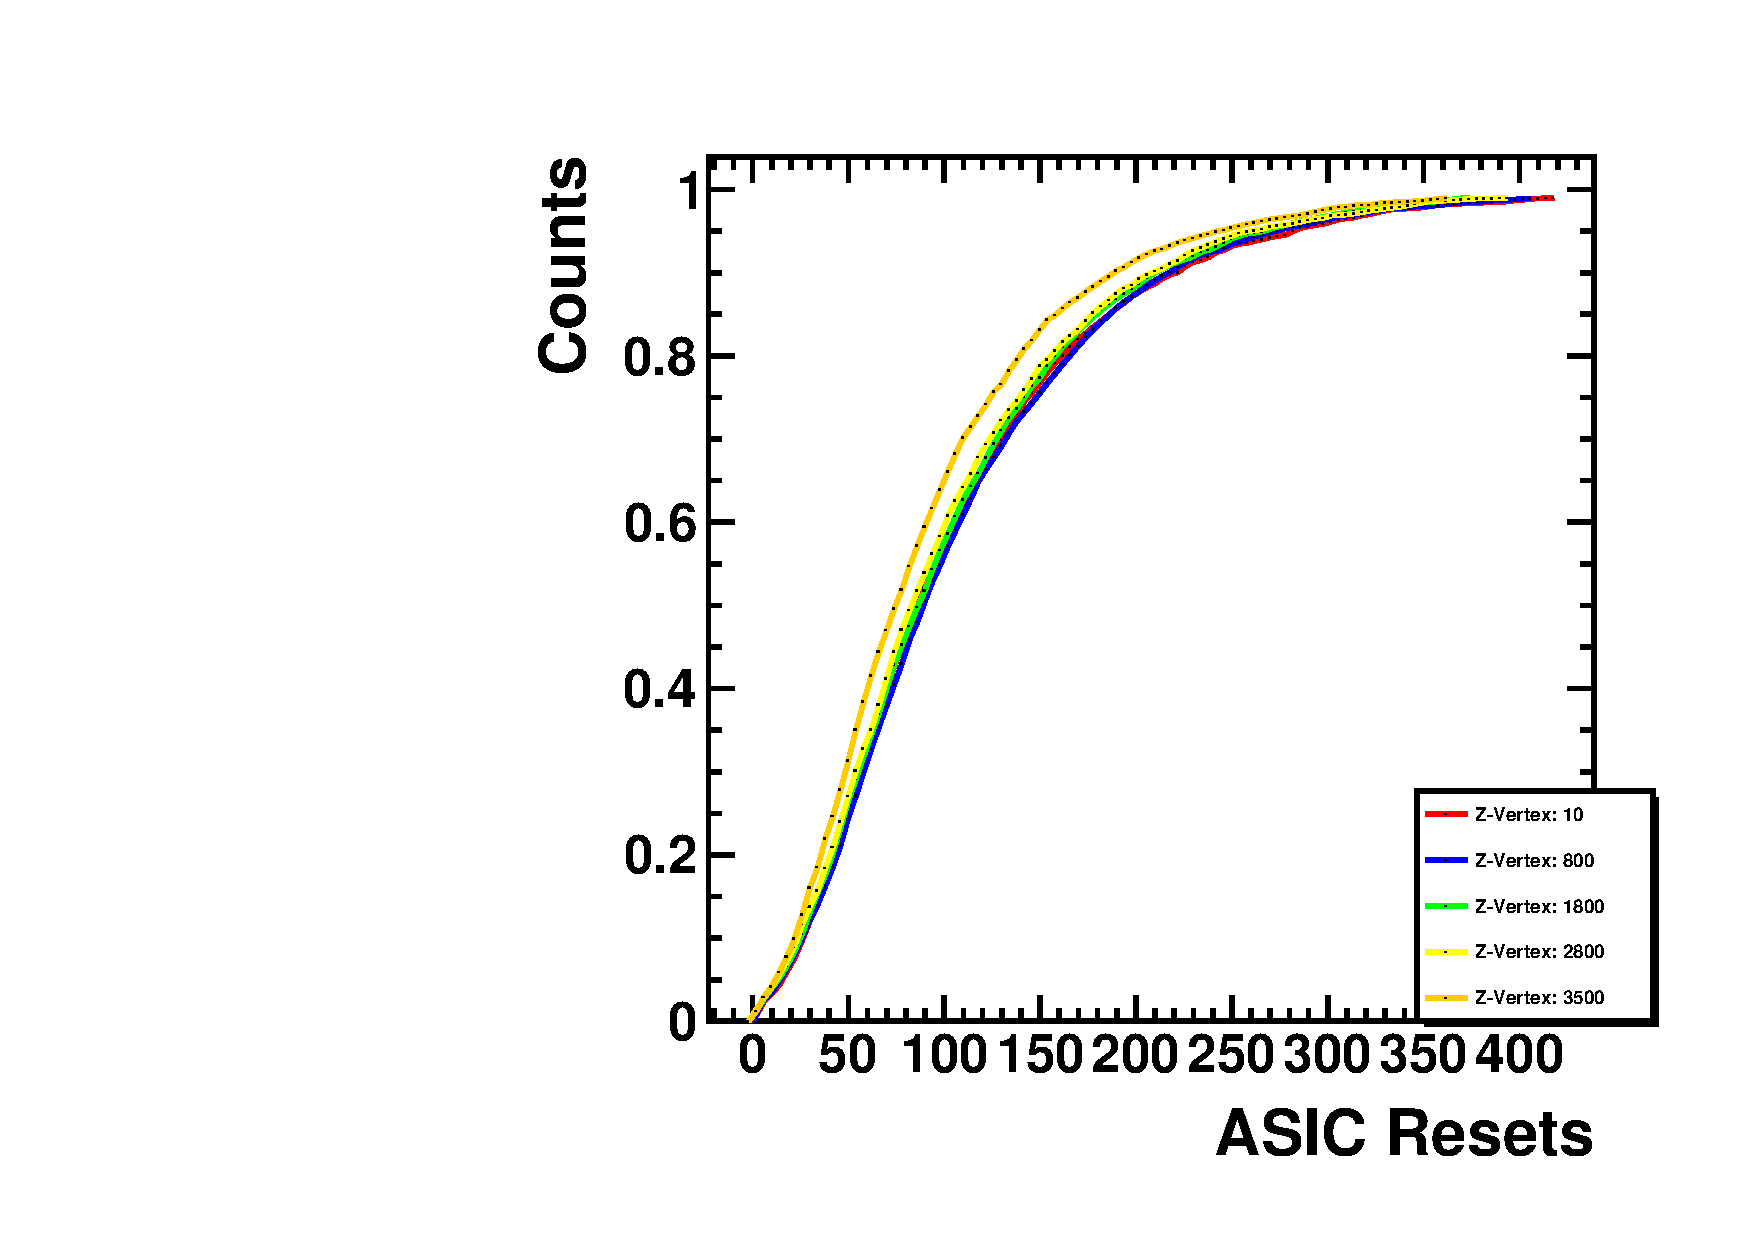
\includegraphics[width=\textwidth]{images/Const_Theta0_ASIC_integral_pdg12_fhc.pdf}
  \caption{Remote FIFO Depths}
\end{subfigure}
\caption{Events for different beam directions for $\nu_{e}$ particle for different momentum directions.}
\label{fig:example_asic_integral_value_constTheta}
\end{figure}


%% example integral of ASIC buffer depths with constant zpos value
\begin{figure}
\centering
\begin{subfigure}{.5\textwidth}
  \centering
  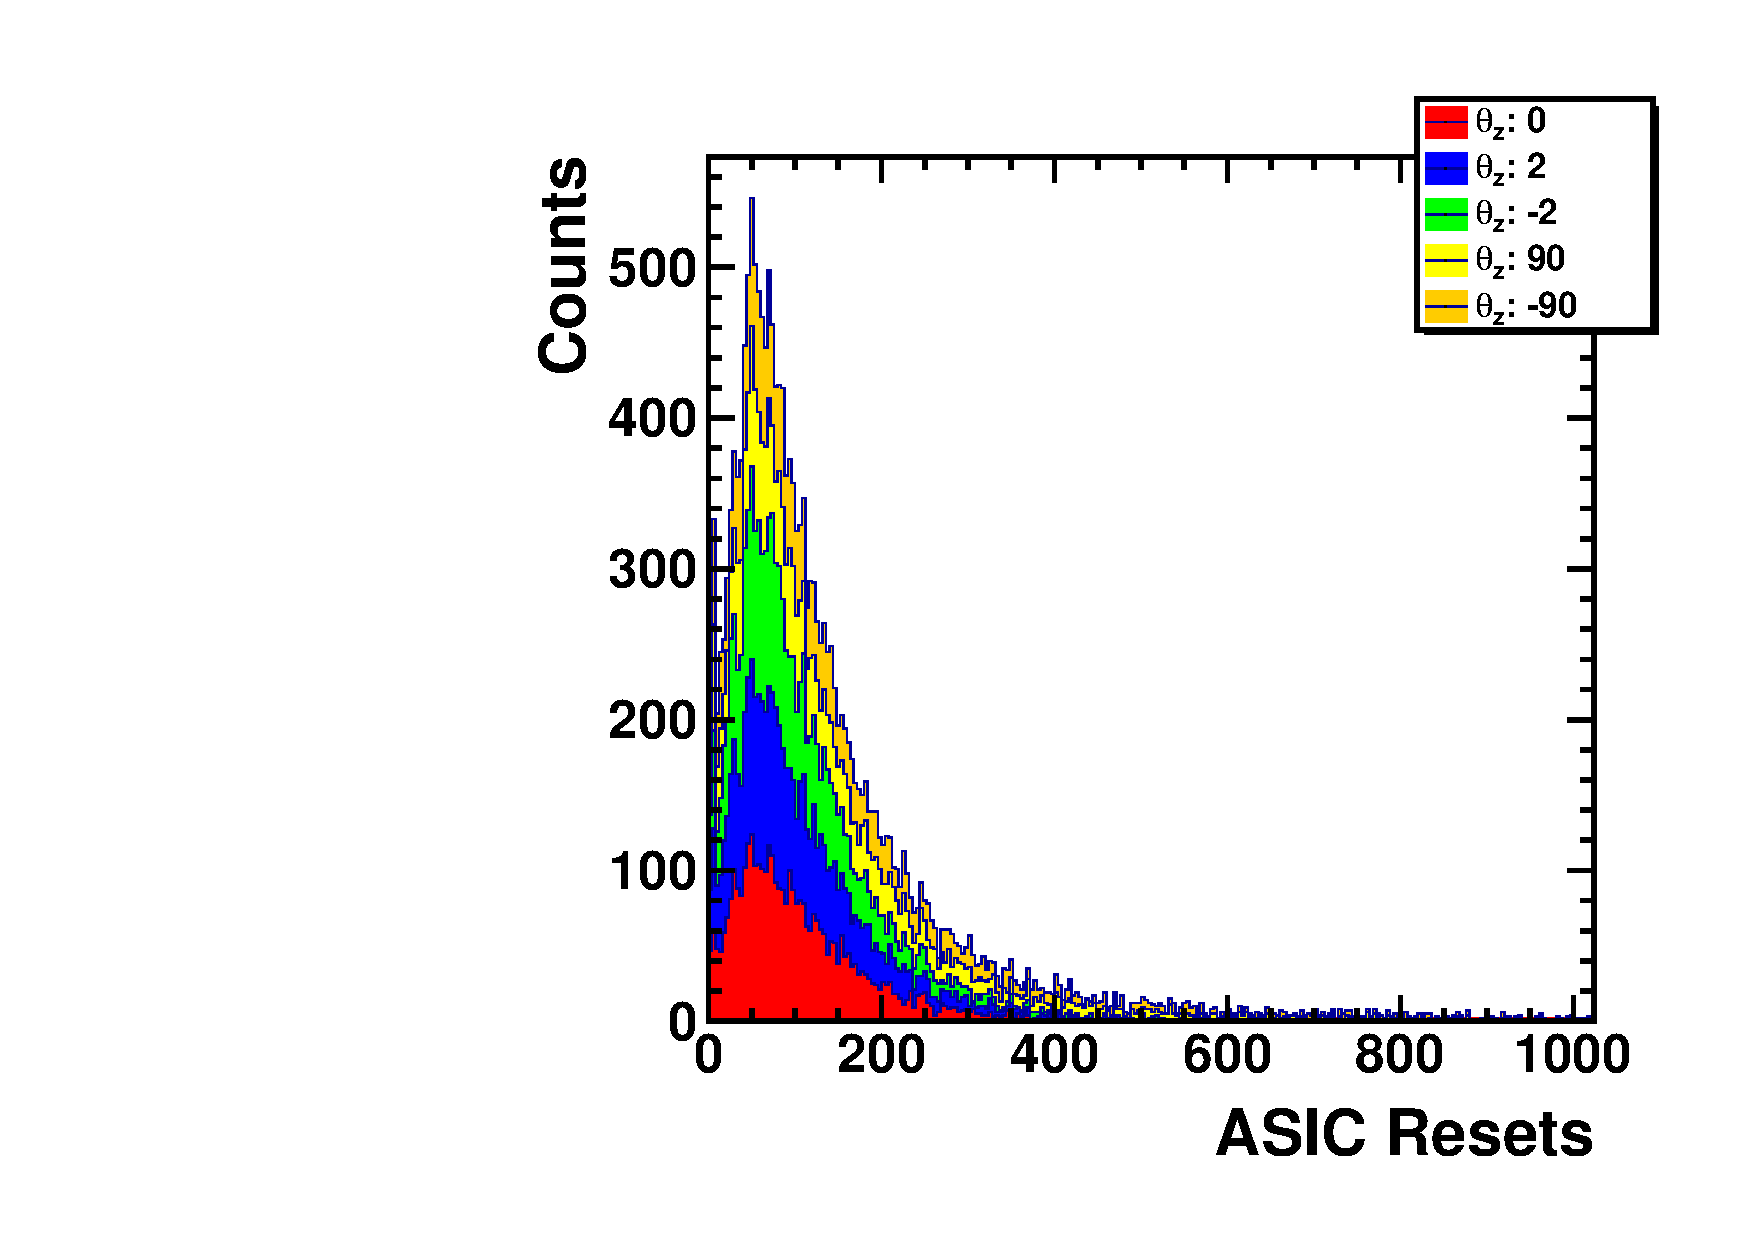
\includegraphics[width=\textwidth]{images/Const_Z180_ASIC_stack_integral_pdg12_fhc.pdf}
  \caption{Stack Of ASIC Buffer depths}
\end{subfigure}%
\begin{subfigure}{.5\textwidth}
  \centering
  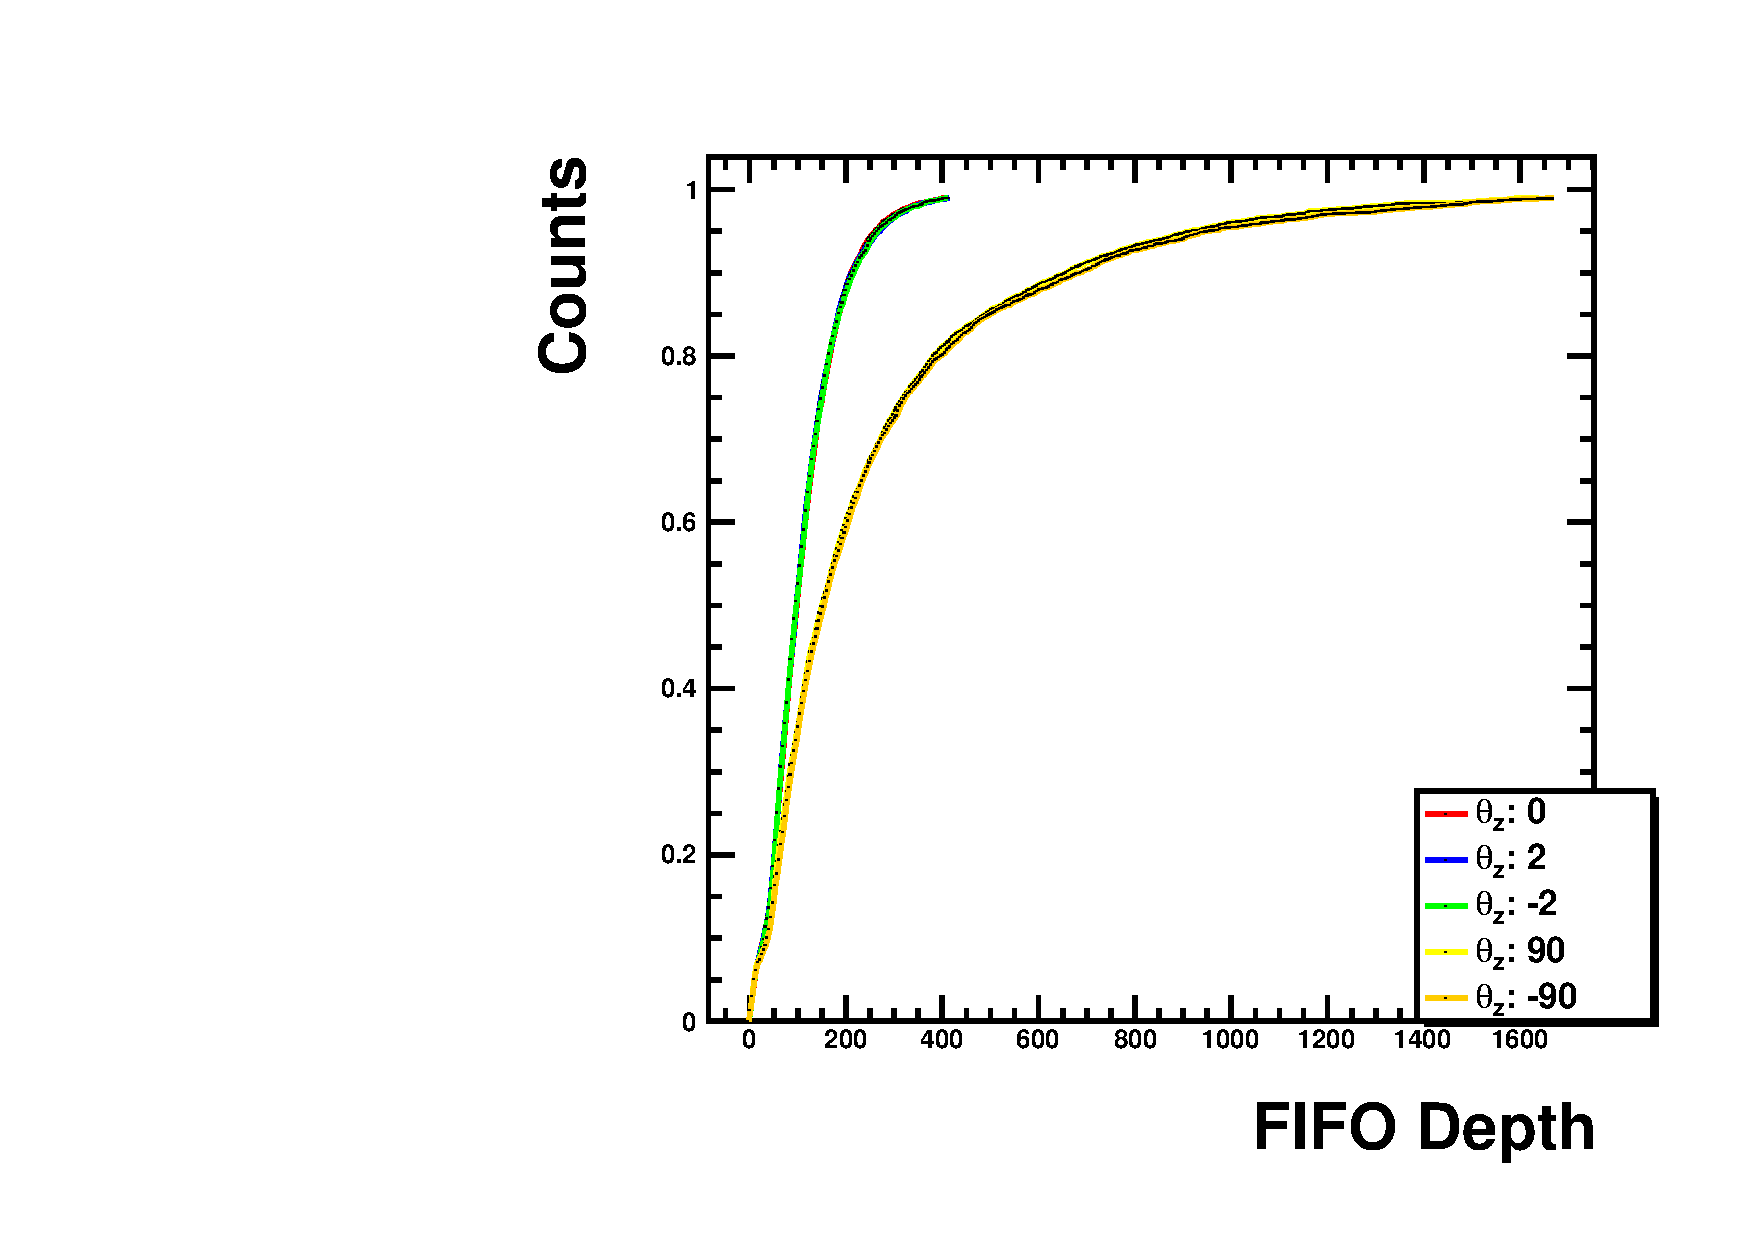
\includegraphics[width=\textwidth]{images/Const_Z180_ASIC_integral_pdg12_fhc.pdf}
  \caption{Integral of ASIC local FIFO depths}
\end{subfigure}
\caption{Integral of the ASIC Buffers.}
\label{fig:example_asic_integral_value_constZpos}
\end{figure}

%% energy comparison for different different zpos and theta values
\begin{figure}
\centering
\begin{subfigure}{.5\textwidth}
  \centering
  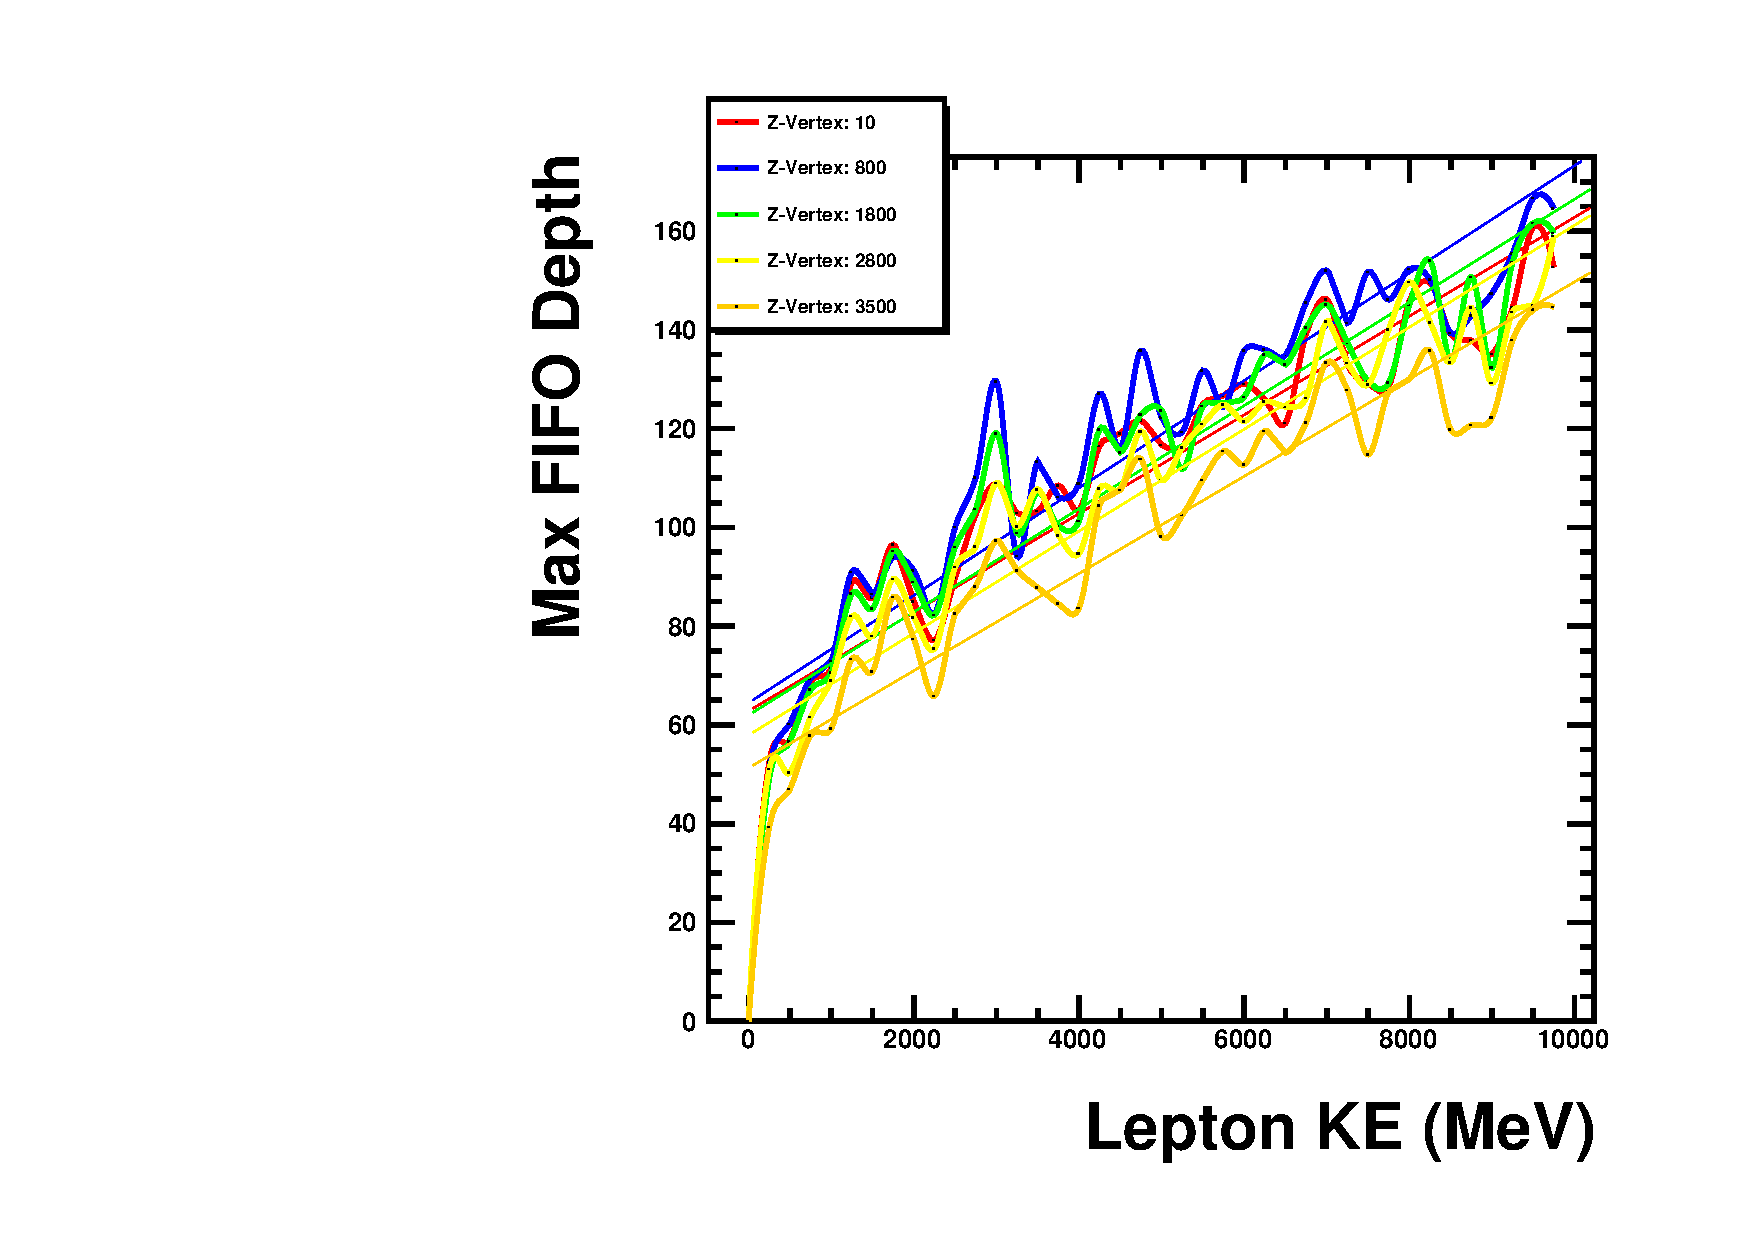
\includegraphics[width=\textwidth]{images/Const_Theta0_ASIC_lepKE_multigraph_pdg12_fhc.pdf}
  \caption{Constant $\theta_{z} = 0$ direction.}
\end{subfigure}%
\begin{subfigure}{.5\textwidth}
  \centering
  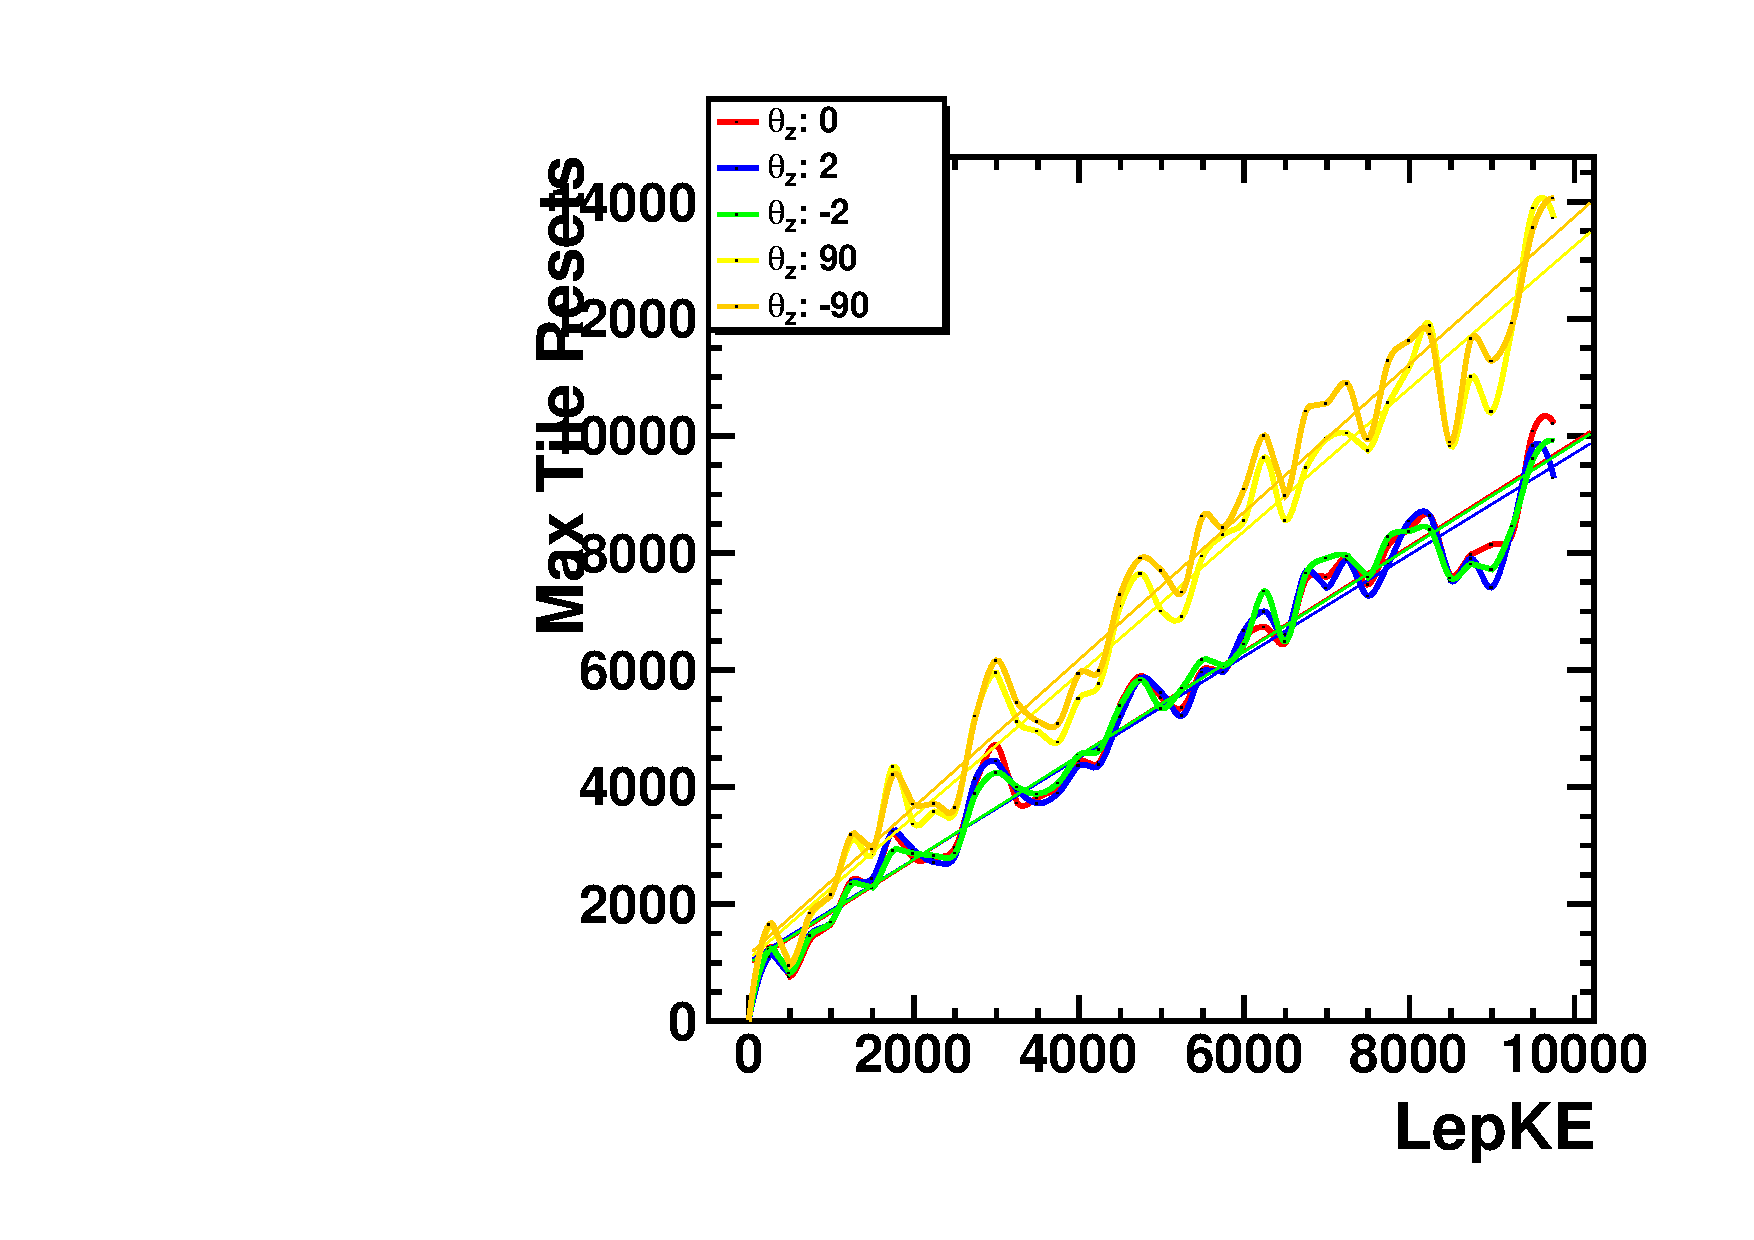
\includegraphics[width=\textwidth]{images/Const_Z180_ASIC_lepKE_multigraph_pdg12_fhc.pdf}
  \caption{Constant Z-Position: $Z = 180\unit{cm}$.}
\end{subfigure}
\caption{Comparison of Buffer depths as a function of energy for different parameters of $\theta_{z}$ and z-position.}
\label{fig:example_asic_energy_comparison}
\end{figure}

%% comparing integral results here
%% 
\begin{figure}
\centering
\begin{subfigure}{.5\textwidth}
  \centering
  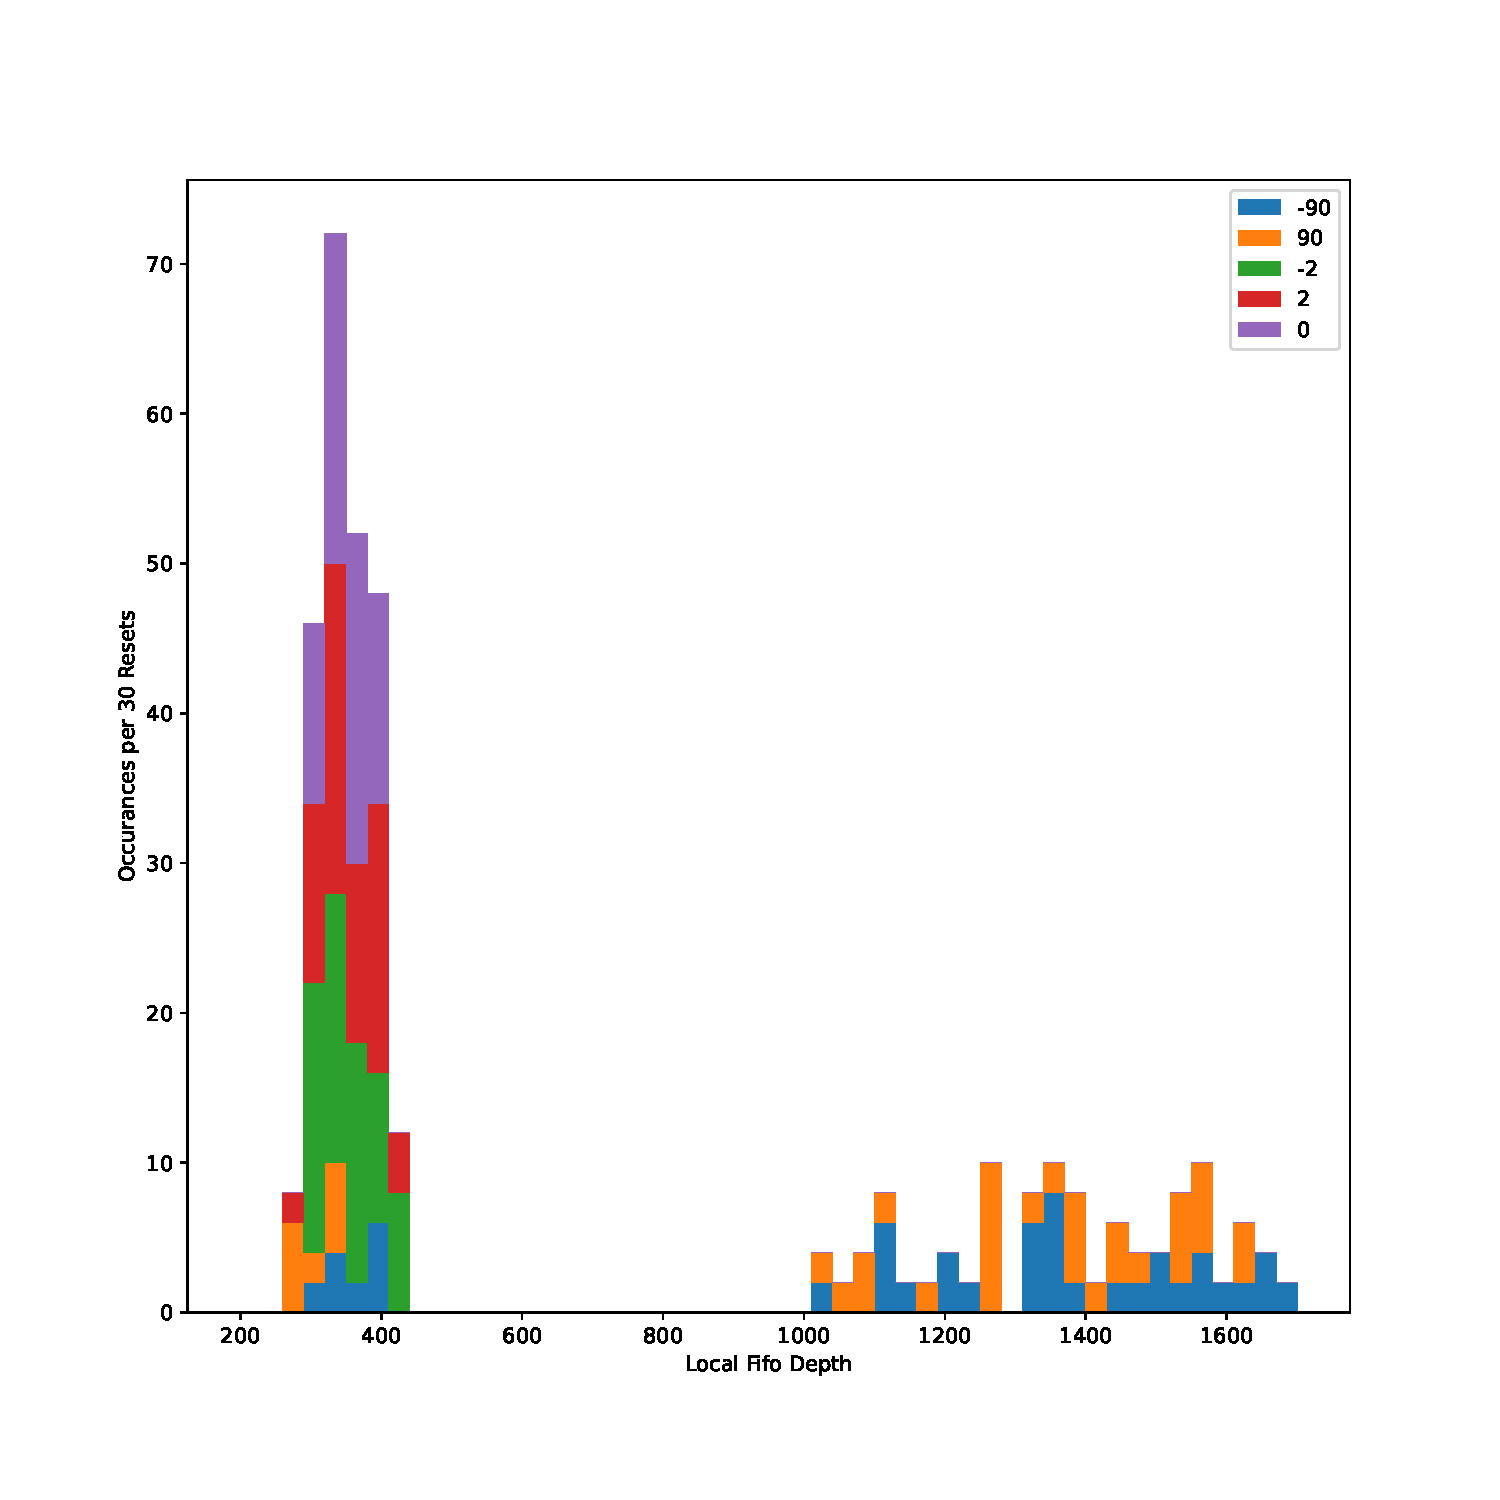
\includegraphics[width=\textwidth]{images/df_theta_cut.pdf}
  \caption{Colored by $\theta_{z}$ direction.}
\end{subfigure}%
\begin{subfigure}{.5\textwidth}
  \centering
  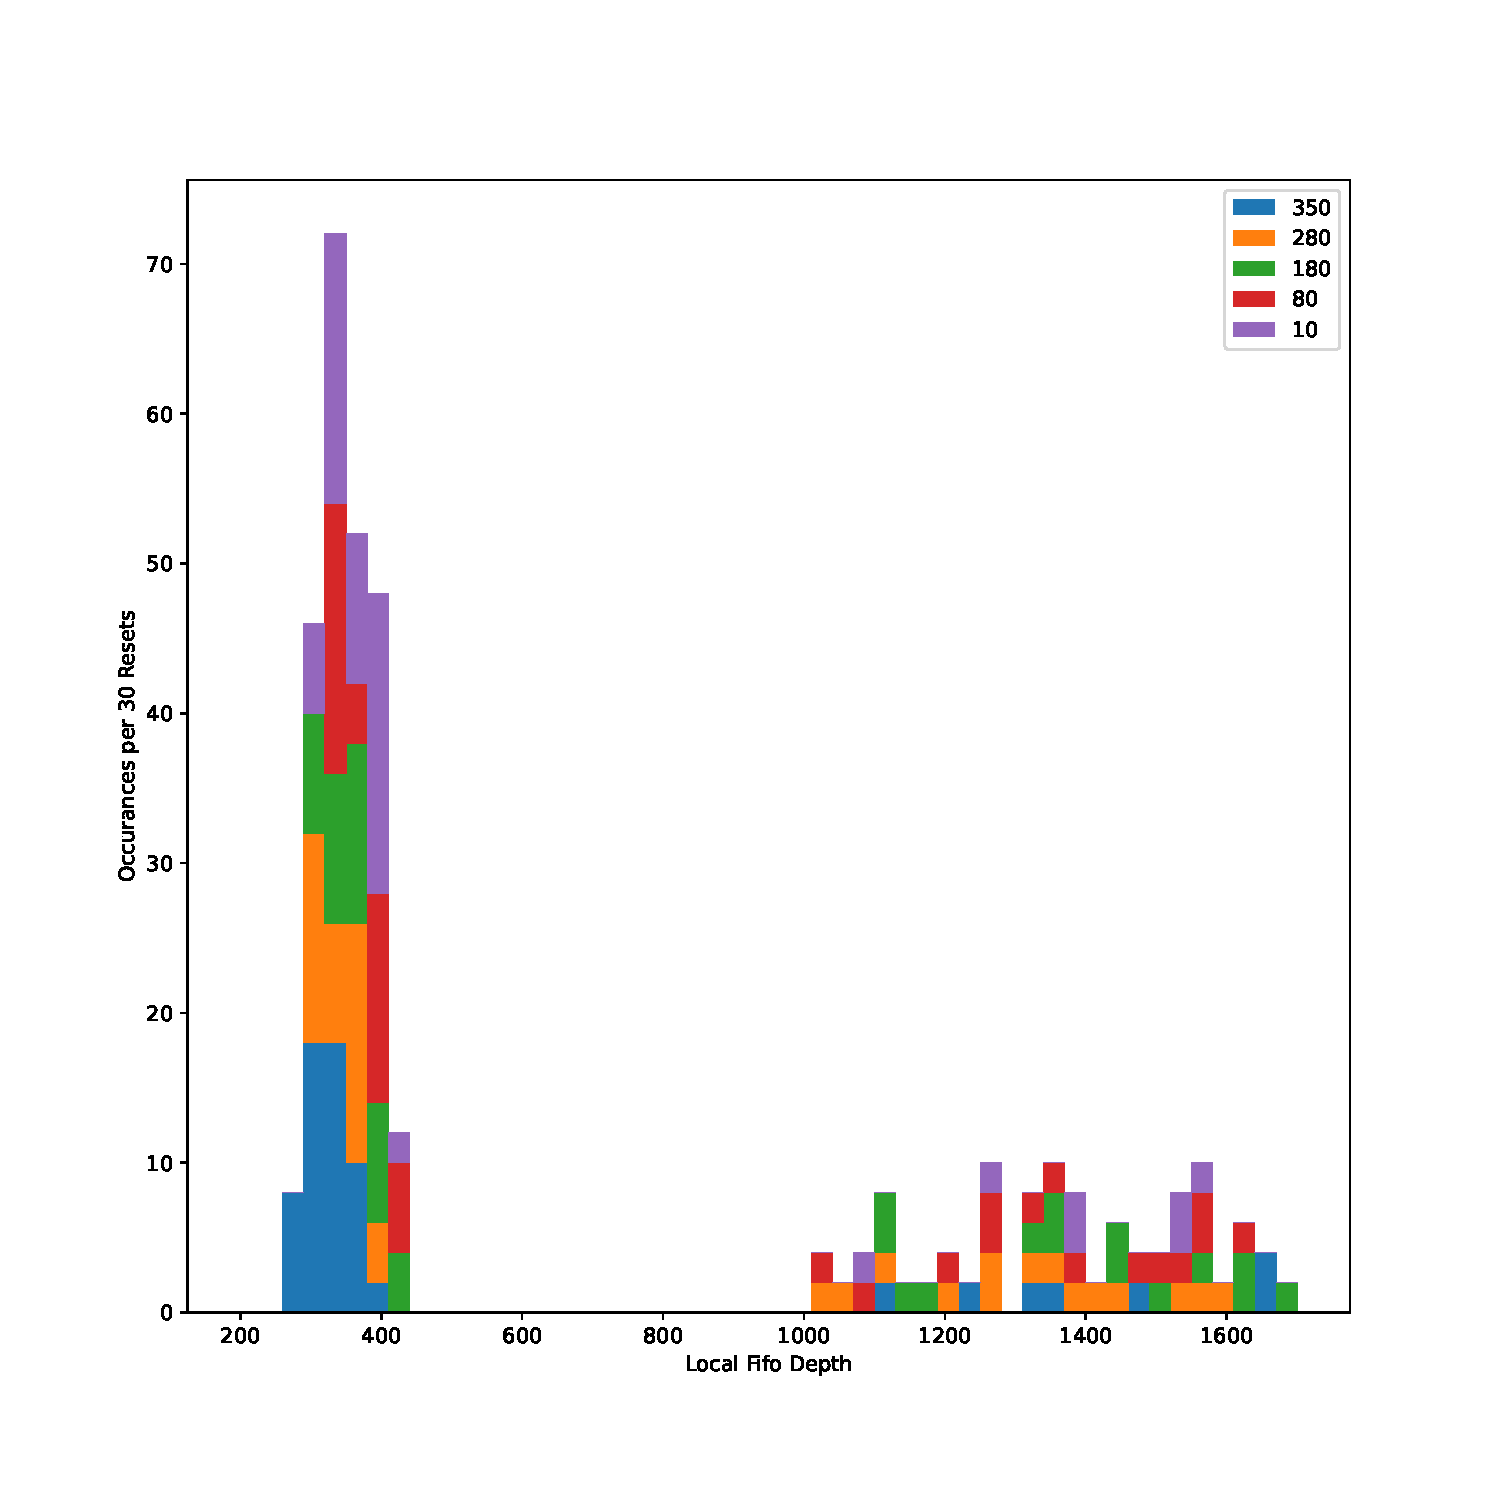
\includegraphics[width=\textwidth]{images/df_zpos_cut.pdf}
  \caption{Colored by Z-position}
\end{subfigure}
\caption{Comparison of Buffer depths as a function of energy for different parameters of $\theta_{z}$ and z-position.}
\label{fig:compare_integral_zpos_theta}
\end{figure}

\begin{figure}
\centering
\begin{subfigure}{.5\textwidth}
  \centering
  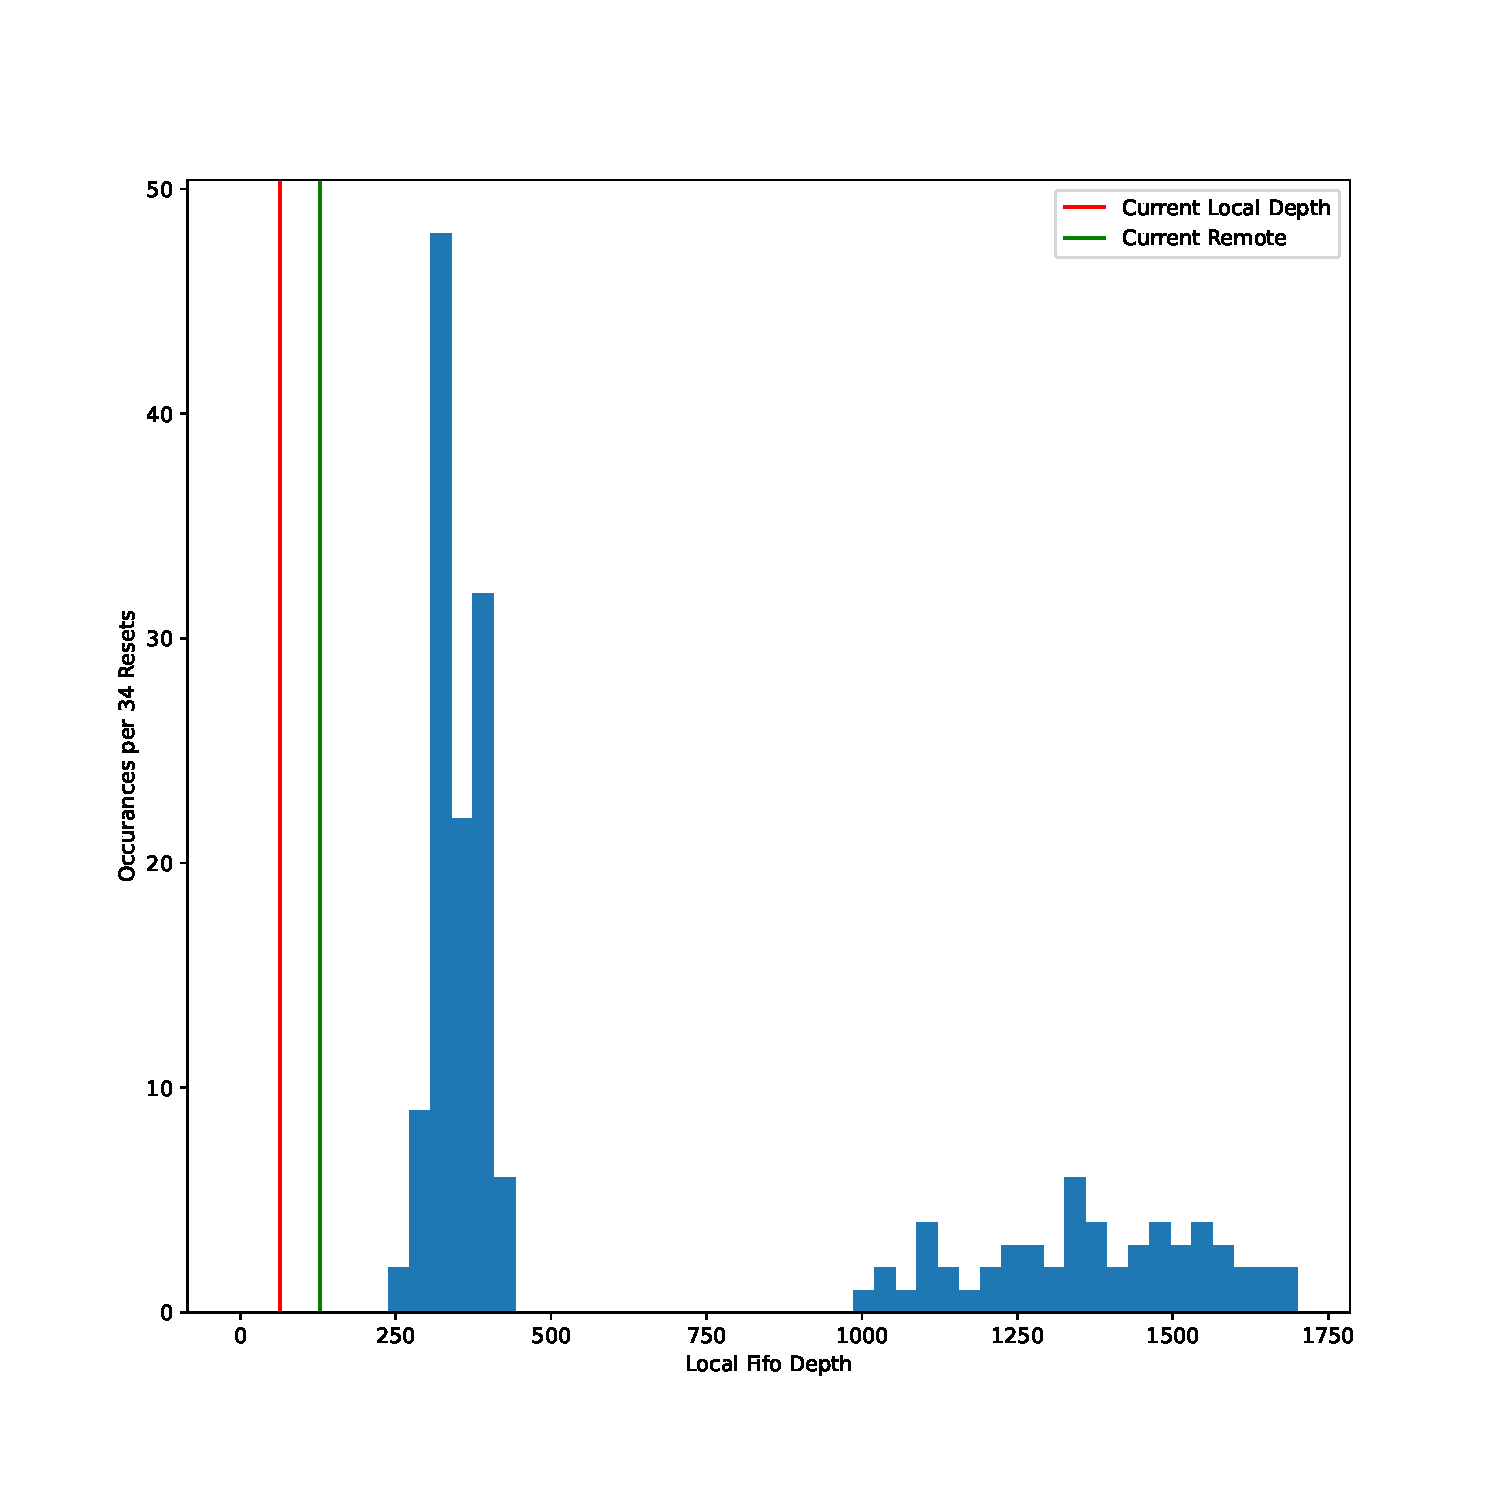
\includegraphics[width=\textwidth]{images/df_nolabel_line.pdf}
  \caption{Comparison of all integrals to current prototype depths.}
\end{subfigure}%
\begin{subfigure}{.5\textwidth}
  \centering
  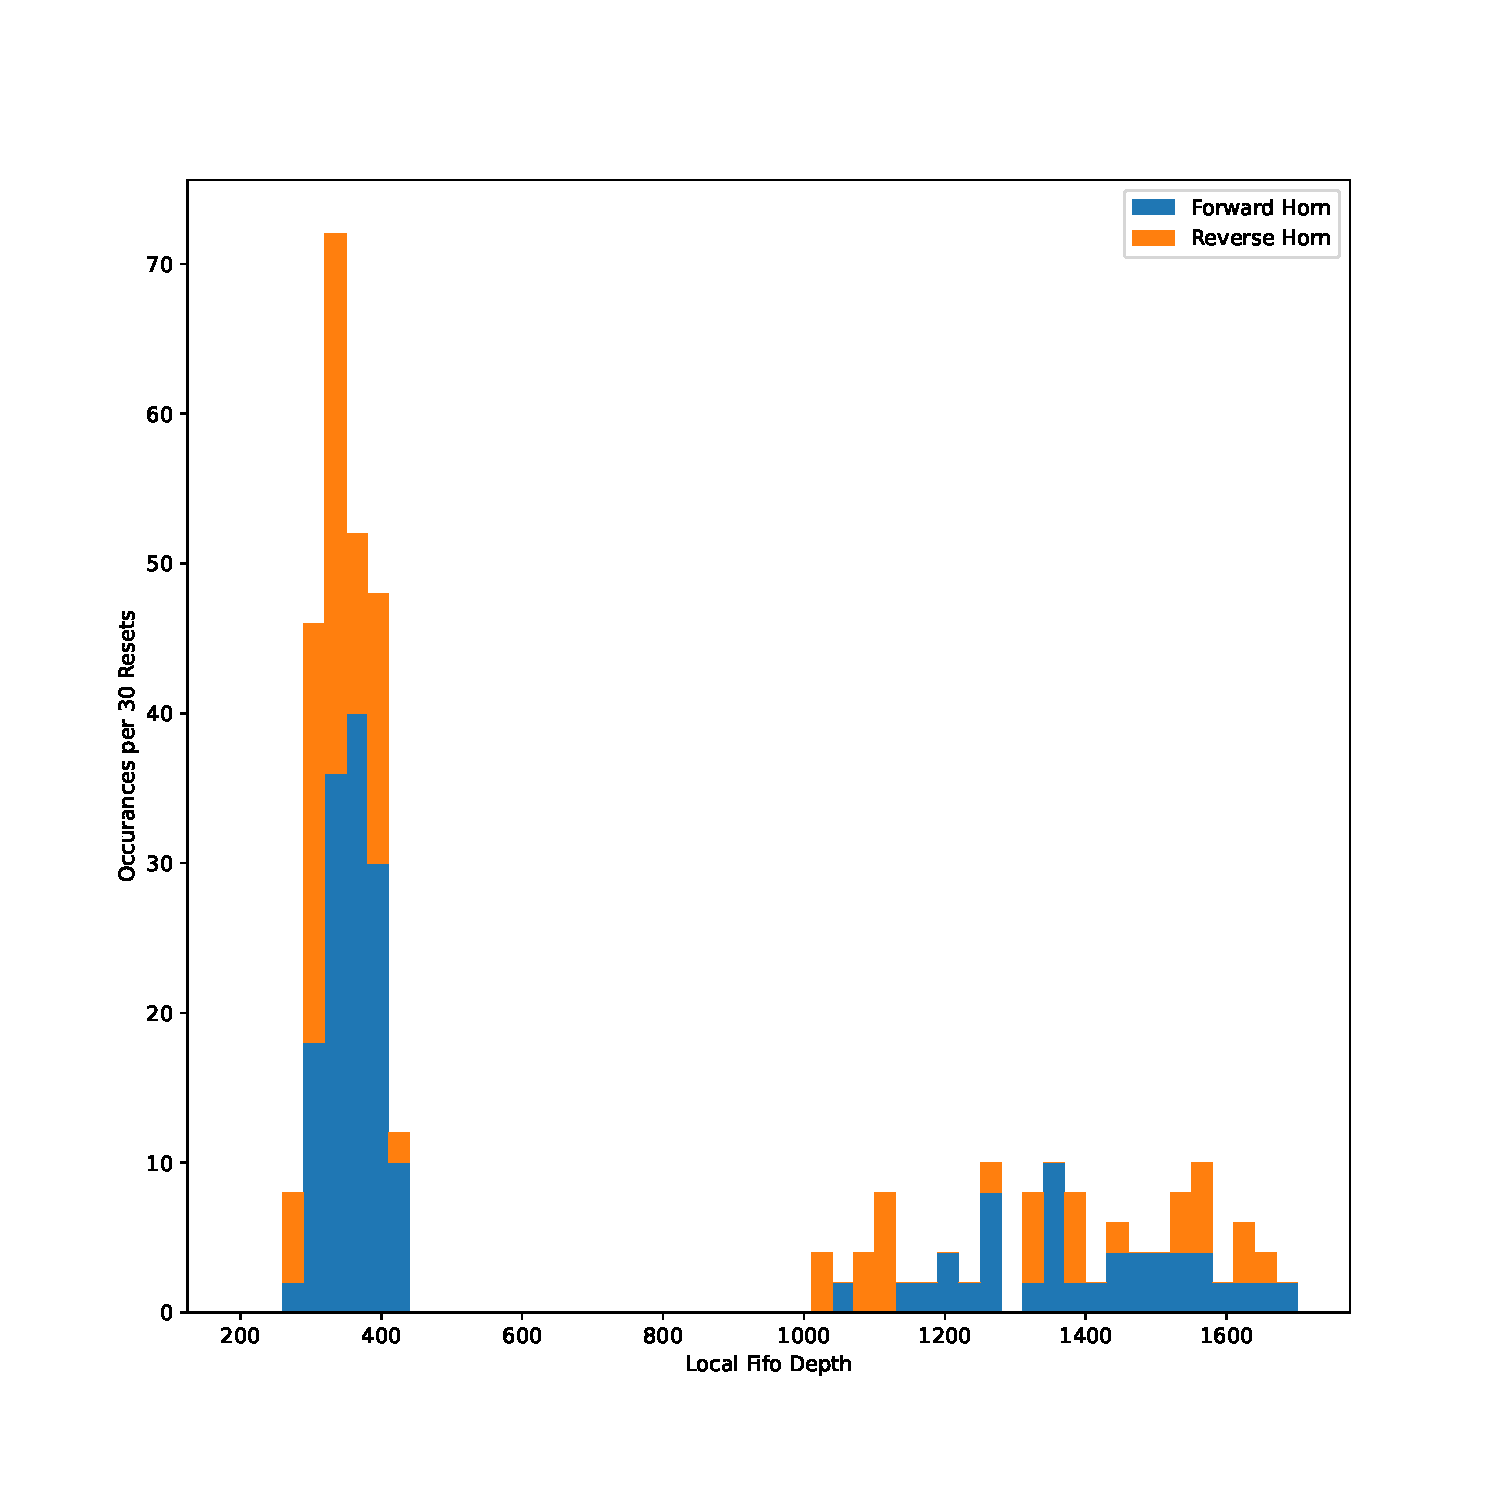
\includegraphics[width=\textwidth]{images/df_horn_cut.pdf}
  \caption{Colored by Z-position}
\end{subfigure}
\caption{Comparison of Buffer depths as in incoming prototype and horn current direction from neutrino beam.}
\label{fig:compare_integral_nolabel}
\end{figure}